% !TeX spellcheck = de_DE

\documentclass{article}

\usepackage[ngerman]{babel}
\usepackage{graphicx}
\usepackage{indentfirst}
\usepackage{hyperref}
\usepackage{geometry}

\graphicspath{ {./images/} }

\makeatletter
\newcommand{\sectionauthor}[1]{
	{\parindent 0em \large \scshape Autor: #1 \par \nobreak \vspace*{2em}}
	\@afterheading
}
\newcommand{\specification}[3]{
	{\parindent 0.5em \hangindent 3em \hypertarget{spec:#1:#2}{\textbf{/#1#2/}} #3 \par \nobreak \vspace*{0.5em}}
}
\makeatother

\title{Bibliothekanwendung - Pflichtenheft}
\date{\today}
\author{
	Ivan Charviakou\\
	León Liehr\\
	Mohamad Najjar\\
	Jonas Picker\\
	Sergei Pravdin
}

\begin{document}

\maketitle
\begin{figure}[h]
	\centering
	\includegraphics[width = 20em]{Dedede}
\end{figure}
\newpage

\tableofcontents
\newpage

\section{Einleitung} %-------------------------------------------------------------------------------------------------
\sectionauthor{Jonas Picker}
Aufbauend auf dem Lastenheft von Christian Bachmaier und Armin Größlinger für ein Bibliothekssystem steckt unser Team, bestehend aus Sergei Pravdin, Ivan Charviakou, León Liehr, Mohamad Najjar und Jonas Picker, mit diesem Pflichtenheft den Rahmen der zu erbringenden Leistungen und verwendeten Technologien bei der Bearbeitung des Auftrags ab. Bei dem zu erstellenden System handelt es sich um eine vereinfachte Form eines Bibliotheksverwaltungssystems mit dem der Anwender das mediale Bibliotheksinventar zentral durchsuchen, kategorisieren und die Nutzung verwalten kann. Das fertige Produkt wird über einen Webbrowser bedient und bietet zahlreiche Anpassungsmöglichkeiten. Das restliche Dokument beinhaltet die genauen Spezifikationen der zu implementierenden Funktionalitäten.
\newpage

\section{Zielbestimmung} %-------------------------------------------------------------------------------------------------
\sectionauthor{Jonas Picker}

\subsection{Musskriterien}
Bei der Produktinstallation setzt der Betreiber den gewünschten Webspace sowie die vom System verwendete Datenbank und den E-Mail-Server. Im laufenden System zählt der Betreiber zu den Administratoren. Technische Maßnahmen sorgen dafür, dass jegliche sensible Information sicher übertragen sowie gespeichert wird und kein unbefugter Zugriff auf zugangsbeschränkte Bereiche der Anwendung durch Dritte erfolgt. Eine unterstützende Bedienanleitung steht für jeden nicht offensichtlichen Aspekt der Anwendung online zur Verfügung.

\begin{flushleft}
\textbf{Administratoren:} In diesen Status werden authentifizierte Benutzer initial vom Betreiber und danach von anderen Administratoren erhoben, dies kann auch rückgängig gemacht werden. Administratoren sind für die Anwendungskonfiguration zuständig, welche das Setzen der institutionsspezifischen Eigenschaften (Logos, Namen, Impressum, Datenschutzerklärung etc.) sowie Variationen des Look \& Feels beinhalten, außerdem bestimmen sie Registrierungsbedingungen und Zugangsberechtigungen für anonyme Nutzer.  Die Definition von Eigenschaften der vom System verwalteten Medien sowie Festlegen ihrer benutzerdefinierten Kategorien, die hierarchisch (bis Tiefe 2) in Verbindung stehen können, wird den Administratoren zusätzlich zur Bearbeitung der Attributwerte einzelner Medieninstanzen ermöglicht. Verwaltungs- und Übersichtsfunktionen zur Ausleihe und Rückgabe von Medien und den damit verbundenen Fristen werden außerdem bereitgestellt. Administratoren können andere Nutzerkonten editieren und löschen, hierfür steht ihnen eine Suchfunktion zur Verfügung. 
\end{flushleft}

\begin{flushleft}
\textbf{Authentifizierte Nutzer:} Nach einer Validierung der E-Mail-Adresse ist ein Nutzer im System registriert und kann sich jederzeit mit seinen Accountdaten anmelden, danach kann diese verändern und er kann sich verfügbare Exemplare von Medien zur Abholung markieren, hierzu steht ihm die im nächsten Paragraph beschriebene Suchfunktion zur Verfügung. Wird das Exemplar innerhalb einer gesetzten Frist abgeholt, gilt es als ausgeliehen und der authentifizierte Nutzer wird per E-Mail automatisch über den Ablauf der Rückgabefrist informiert. Ein angemeldeter Benutzer kann seinen Account selbstständig löschen und sich jederzeit abmelden.
\end{flushleft}

\begin{flushleft}
\textbf{Anonyme Nutzer:} In der Standartkonfiguration erlaubt das System Besuchern des Webspaces, neben der Registrierungsmöglichkeit, den Zugriff auf eine Suchfunktion sowie das Herunterladen/Lesen öffentlich zugänglicher Medien. Diese Berechtigungen können von Administratoren auf die Registrierungsmöglichkeit reduziert werden. Die Suchfunktion beinhaltet eine graphische Darstellung der gesamten Kategoriehierarchie und die Möglichkeit sowohl nach Medien als auch nach deren Attributen zu suchen und diese Suche nach Kategorien zu filtern. Eine Detailansicht zu gefundenen Medien steht ebenfalls zur Verfügung.
\end{flushleft}

\subsection{Wunschkriterien}

\begin{flushleft}
\textbf{Administratoren:} Beim der Zuweisung der Kategorien für Medien ist die Hierarchietiefe unbeschränkt. Zusätzlich besitzen Administratoren die Möglichkeit, einzelnen registrierten Nutzer ohne Administratorberechtigungen die Ausleihberechtigung zu entziehen bzw. zu verleihen. Hierzu gibt es eine gesammelte Ansicht der noch nicht freigeschalteten Accounts.
\end{flushleft}

\begin{flushleft}
\textbf{Authentifizierte Nutzer:} Die Accountdaten des Nutzers können mit einem Avatarbild versehen werden, außerdem besteht die Möglichkeit die mit diesem Account ausgeliehenen/reservierten Medienexemplare einzusehen. Angemeldete Benutzer können alternativ zur Abholungsmarkierung eine Reservierung beantragen, sollten alle Exemplare eines Mediums ausgeliehen sein. Der Nutzer wird dann über den vorraussichtlichen Rückgabetermin des reservierten Exemplars informiert, und bei Abholungsmöglichkeit per E-Mail benachrichtigt. Er kann außerdem seine Reservierung zurückziehen.
\end{flushleft}

\begin{flushleft}
\textbf{Schaltermitarbeiter:} Mit dieser Nutzerrolle haben Mitarbeiter der Bibliothek die Möglichkeit, zur Abholung markierte Exemplare gesammelt einzusehen und abzuarbeiten, indem sie den Abholstatus verändern. Außerdem können sie zurückgegebene Ausleihen wieder als verfügbar markieren. Zusätzlich ist es ihnen möglich Attributwerte für Medien und Exemplare zu editieren.
\end{flushleft}

\subsection{Abgrenzungskriterien}

Der Hauptfokus des Produkts liegt auf der Organisation und Verwaltung von Medien und Nutzern der Bibliothek, Funktionalitäten zum Erwerben und Verwalten von Lizenzen und/oder neuen Medien stehen nicht zur Verfügung. Die Abwicklung oder Verfolgung der Kundenzahlungen für Mitgliedsbeiträge, Medienerwerb o.ä. ist ebenfalls nicht im System integriert. Es besteht keine Möglichkeit, andere Bibliotheksmanagementsysteme oder Literaturenzyklopädien mit dieser Software zu verknüpfen. Das System ist für die klassische Benutzung über einen mit Tastatur, Maus und Bildschirm ausgestatteten PC/Laptop gedacht, mobile Geräte oder barrierefreie Benutzung werden begrenzt bis gar nicht unterstützt.

\newpage

\section{Produkteinsatz} %-------------------------------------------------------------------------------------------------
\sectionauthor{Sergei Pravdin}
\subsection{Anwendungsbereich}
Das Bibliothekssystem wird hauptsächlich für die allen Typen der Bibliotheken (Universitätsbibliotheken, staatliche Bibliotheken usw.) entwickelt. Aber das System kann unter anderem in einem beliebigen Unternehmen, das eine Menge der Medien verwalten möchte, eingesetzt werden. Das System lässt eine Menge der Medien nicht nur im geöffneten Modus, sondern auch im geschlossenen Modus verwalten.
\subsection{Zielgruppen}
Das System ist auf Personen ohne fachspezifische Kenntnisse ausgerichtet, die sich für Medien interessieren. Die Benutzeroberfläche sind in Deutsch erstellt, deshalb sind die Deutschkenntnisse für die Anwendung des Systems vorausgesetzt. Optional kann das System in Zukunft mit mehreren Sprachen erweitert werden.
\subsubsection{Administrator}
Das System hat mindestens einen Administrator, der das System konfiguriert kann. Für die Konfigurierung sind keine fachspezifische Kenntnisse nötig, weil das System die Anwendungsschnittstelle für Administratoren hat. Die Registrierung, die Verwaltung der Medien und die graphische Darstellung des Systems werden von einem Administrator eingestellt.
\subsubsection{Personalarbeiter}
Das System hat Personalarbeiter, die die Medien den Benutzern abgeben und zurücknehmen können.
\subsubsection{Angemeldete Benutzer}
Angemeldete Benutzer haben nicht nur einen Zugriff zu der Kataloge und zum Suchen der Medien, sondern auch einen Zugriff zur Reservierung und zur Buchung der Medien. Angemeldete Benutzer können ihre eigene Konten einstellen, ändern und löschen. Angemeldete Benutzer können sich abmelden.
\subsubsection{Anonyme Benutzer}
Falls sich das System in keinem geschlossenen Modus befindet, haben anonyme Benutzer einen Zugriff zur Medien-Kataloge, somit können sie die Medien nach Attributen mit dem Suchfeld suchen. Anonyme Benutzer können sich registrieren oder anmelden, falls sie ein Konto haben. Eine gültige E-Mail-Adresse wird für eine Registrierung eines Benutzers vorausgesetzt. 
\subsection{Betriebsbedingungen}
Das System ist eingesetzt und von einem Administrator eingestellt. Das System ist kontinuierlich erreichbar. Die Erreichbarkeit wird von einem Webserver, einer Verbindung mit einer Netz und einer Datenbank sichergestellt, die von einem Betreiber bereitgestellt werden. Die Aufsicht und regelmäßige Backups des Systems von den Administratoren ist empfehlenswert. Bei Wartungen und Updaten ist das System nicht erreichbar, deshalb ist es empfohlen entsprechende Meldungen über eine eingeplante Wartung von einem Administrator den Benutzern im Voraus zu schicken. Bei technischen Fehlern und Bugs sollen Benutzer einen Administrator kontaktieren.
\newpage

\section{Produktumgebung} %-------------------------------------------------------------------------------------------------
\sectionauthor{Jonas Picker}

\subsection{Software}

Im folgenden Abschnitt werden Softwareabhängigkeiten und Kompatibilitäten des Produkts beschrieben.

\begin{itemize}
\item \underline{\textbf{Clientsoftware}}: \linebreak
Die Applikation wird über einen Webbrowser benutzt, dieser sollte die Darstellung in den Auszeichnungssprachen HTML, Version 5 und CSS, Level 3 unterstützen, sowie die Kommunikation mit dem HTTP/2-Protokoll. Die Unterstützung von JavaScript (ECMAScript 2020) im Browser wird empfohlen. Explizit getestet werden die aktuellen Versionen der weit verbreiteten Browser: Google Chrome, Version: 88.0; Mozilla Firefox, Version: 85.0 und Apple Safari, Version: 14.0.3. Da HTML 5 (und CSS) jedoch seit einem guten Jahrzehnt als Web-Standart gilt, ist weitreichende Abwärts-Kompatibilität bei den meisten Browsern zu erwarten.  

\item \underline{\textbf{Serversoftware}}: \linebreak
Auf dem Server muss die Laufzeitumgebung 'Java Virtual Maschine' verfügbar sein, zudem benötigt die Anwendung den Java Enterprise Applikationsserver Apache Tomcat, Version 10.0.x, dieser bringt zwar bei der Installation eine Java Laufzeitumgebung mit sich, es wird jedoch empfohlen, das komplette 'Development Kit' OpenJDK 16 herunterzuladen und bei Tomcat zu registrieren um Kompatibilitätsprobleme zu vermeiden. Außerdem muss ein E-Mail-Server bereit stehen, der das SMTP-Protokoll unterstützt. Die verwendete Datenbank muss das objektrelationale Datenbankmanagementsystem PostgreSQL, Version 13 benutzen, zusätzlich muss die Datenbank über ein gültiges SSL-Zertifikat verfügen um Datenübertragungen mit dem TLS-Protokoll zu ermöglichen. Die Installation der JVM/Tomcat, das Aufspielen der Anwendung sowie die Registrierung der Datenbank und des E-Mail-Servers werden in einem Installationsdokument beschrieben.
\end{itemize}

\subsection{Hardware}

Hier werden die geschätzen Rahmenbedingungen der Hardware für einen reibungslosen Betrieb aufgelistet, obwohl konkretere Messungen erst mit der Fertigstellung des Produkts möglich sind, skalieren die verwendeten Technologien, und damit die Kapazitäten der Anwendung, prinzipiell mit dem Aufstocken der Rechenleistung (am Server) mit. Sollten die Rahmenbedingungen unterschritten werden, ist ein Betrieb meistens immer noch möglich, jedoch nicht garantiert.

\begin{itemize}
\item \underline{\textbf{Clienthardware}}: \linebreak
Die Bedienung der Anwendung über die oben beschriebenen Browsertypen setzt voraus, dass Clientrechner die jeweiligen Hardwareanforderungen für deren Betrieb erfüllen.
\item \underline{\textbf{Serverhardware}}: \linebreak
Die Mindestanforderungen zum Betreiben einer Datenbank unter PostgreSQL bzw. eines Applikationsservers unter Tomcat reichen für einen sinnvollen Betrieb der Anwendung unter Last nicht aus, wie oben erwähnt sollten die der Anwendung zur Verfügung stehenden Ressourcen mit der Nutzerzahl in Relation stehen. Als Referenzplattform zum Betreiben der Anwendung dient der im Abschnitt 'Entwicklungsumgebung' beschriebene Rechner 'schratz' für Datenbank und Server gleichermaßen.
\end{itemize}

\subsection{Schnittstellen}

\begin{itemize}
\item \underline{\textbf{Clientenschnittstellen}}: \linebreak
Die notwendigen Mensch-Maschine Schnittstellen zum Benutzen der Anwendung über einen Browser sind: Bildschirm, Tastatur. Die Benutzung einer Maus oder vergleichbare Cursorsteuerung wird dringend empfohlen. Die Verifizierung eines neuen Benutzers bei der Registrierung im System wird über eine gültige E-Mail-Adresse abgewickelt, folglich muss der Nutzer Zugriff auf ein E-Mail-Konto besitzen. Der Browser des Klienten muss beim Benutzen über eine konstante Anbindung an das Internet verfügen, eine außergewöhnlich hohe Bandbreite ist nicht erforderlich.
\item \underline{\textbf{Serverschnittstellen}}: \linebreak
Der Server muss über notwendige Mensch-Maschine Schnittstellen zur initialen Installation der Anwendung und ihrer Softwareabhängigkeiten verfügen. Auch benötigt er eine konstante Anbindung an das (Intra- und) Internet, um Klientenanfragen beantworten, den E-Mail-Server kontaktieren und Datenbankanfragen absetzen zu können. Die Datenbank kann sich auf dem gleichen Gerät wie der Server, seperat davon im Netzwerk oder geographisch getrennt 'im Internet' befinden. Sie muss jedoch vom Server aus über einen Hostnamen ansteuerbar sein, je nach Realisierung ist dazu ein VPN-Tunnel notwendig. 
\end{itemize}

\newpage

\section{Produktfunktionen} %-------------------------------------------------------------------------------------------------
\sectionauthor{Ivan Charviakou}
In der folgenden Aufführung unterscheidet man zwischen Administratoren, Schaltermitarbeiter, registrierten Nutzern, angemeldeten Nutzern, und anonymen Nutzern.
Hierbei sind alle angemeldeten Nutzer zwangsweise auch registrierte Nutzer. Trotzdem kann ein registrierter Nutzer vor einer Authentifikation anonymer Nutzer sein.
Ferner ist die Unterscheidung zwischen einem Administrator und Schaltermitarbeiter nur dann zu treffen, wenn die Rolle des Schaltermitarbeiters optional umgesetzt wird.
Ansonsten sind alle Funktionen, die in dieser Aufführung nur einem Schaltermitarbeiter zugeordnet sind, dem Administrator zuzuordnen.
	\subsection{Nutzerverwaltung}
		\subsubsection{Administrator}
			\specification{F}{10}{Es ist einstellbar, ob anonyme Nutzer Lesezugriff auf den OPAC haben.}
			\specification{F}{20}{Es können eine oder mehrere Email-Domäne angegeben werden, mit denen neue Registrierungen durchgeführt werden dürfen.}
			\specification{F}{30}{Die Registrierung eines neuen Nutzers ist möglich.}
			\specification{F}{40}{Die Nutzerdaten und Rolle aller Nutzern, insbesondere auch die eines Administrators, sind änderbar. Die eigene Rolle ist aber unänderbar. }
			\specification{F}{50}{Ein registrierter Nutzer kann gelöscht werden.}
			\specification{F}{60}{Es kann ggf. mit Angabe von Nutzerattributen nach Nutzern gesucht werden.}
			\specification{W}{70}{Nicht-administrative Benutzerkonten können von weiterer Ausleihe gesperrt und entsperrt werden.}
			\specification{W}{80}{Die Liste von gesperrten Nutzerkonten ist aufrufbar.}
		\subsubsection{Anonyme Nutzer}
			\specification{F}{90}{Wenn von Administratoren freigeschaltet, ist eine Registrierung mit Namen, Adresse, und Email-Adresse möglich. 
				Dabei gilt sie nur dann als abgeschlossen, wenn auf den Link zugegriffen wird, der per Email an die angegebene Email-Adresse geschickt wurde. }
		\subsubsection{Registrierte Nutzer}
			\specification{F}{100}{Es ist möglich, sich mit dem Benutzernamen und Kennwort ins System einzuloggen. Beim Erfolg handelt es sich dann um einen angemeldeten Nutzer. }
			\specification{F}{110}{Bei erfolgreicher Anmeldung, ist es möglich, sich auszuloggen. Beim Erfolg handelt es sich dann um einen anonymen Nutzer. }
		\subsubsection{Angemeldete Nutzer}
			\specification{F}{120}{Bis auf die Email-Adresse ist es möglich, die eigenen Nutzerdaten zu ändern. }
			\specification{F}{130}{Das Löschen des eigenen Nutzerkontos ist möglich.}
			\specification{W}{140}{Es kann ein Profilbild hochgeladen werden.}
		\subsubsection{Alle Nutzer}
			\specification{F}{150}{Bei Fehlerhafter Texteingabe zu einem Formular werden alle Felder auf Korrektheit geprüft. Alle Fehler werden dem Nutzer angezeigt. }
	\subsection{Navigation \& Suche}
		\subsubsection{Alle Nutzer}
			\specification{F}{160}{Es ist möglich, mit Texteingabe nach einer Medien-Kategorie zu suchen. }
			\specification{F}{170}{Nach Auswahl einer Kategorie aus einer Baum-Darstellung von allen Kategorien, ist eine Liste von allen darin enthaltenen Medien sichtbar. }
			\specification{F}{180}{Mit Eingabe von Kategorie, Medien-Typ, und jeweiligen Attributen kann eine Suche durchgeführt werden. }
			\specification{F}{190}{Zu einem Medium ist die Liste aller Exemplaren aufrufbar. }
			\specification{F}{200}{Für alle Tabellen ist der Datensatz nach individuellen Spalten auf Anclick ab- und aufsteigend sortierbar. }
			\specification{F}{210}{Die Seite mit Kontaktinformation bzw. Impressum ist aufrufbar. }
			\specification{F}{220}{Alle Tabellen verwenden ggf. Pagination. Insbesondere werden per Default bis zu 20 Datensätzen pro Seite angezeigt. 
				Mit entsprechenden Knöpfen kann man ggf. nach vorwärts und rückwärts blättern. }
			\specification{W}{230}{Es kann für eine Tabelle eingestellt werden, wie viele Datensätze pro Pagination-Seite angezeigt werden. }
	\subsection{Ausleihe \& Rückgabe}
		\subsubsection{Administrator}
			\specification{F}{240}{Der Zeitabstand zwischen dem automatischen Versenden einer Email-Mahnung und der Rückgabefrist für einen beliebigen Exemplar ist setzbar.
				Dieser Wert gilt dann global für alle neue Ausleihvorgänge. Zu beachten ist, dass für einen Vorgang mit einem Ausleihdauer, der kürzer als dieser Wert ist, keine Email-Mahnung versendet wird. }
			\specification{F}{250}{Der Zeitabstand zwischen der Initiierung eines Ausleihvorgangs durch einen Nutzer und dem Abschluss dieser Initiierung durch einen Personalarbeiter oder Administrator ist setzbar.
				In dieser Zeit ist das Exemplar zur Abholung markiert. Zu beachten ist, dass das ausgewählte Exemplar nach Überschreiten dieser Zeit wieder allen Nutzer zu Verfügung steht. }
			\specification{F}{260}{Die Rückgabefrist für ist für alle Ausleihvorgänge setzbar. Dabei darf die Frist nicht in der Vergangenheit liegen. }
			\specification{F}{270}{Die maximale Ausleihdauer ist global, für einen bestimmten Medium, oder für einen bestimmten Nutzer setzbar.
				Wenn bei einem Ausleihvorgang mehrere Werte vorhanden sind, wird zuerst der Nutzerwert, danach der Mediumwert, und als letztes der globale Wert beachtet. }
			\specification{F}{280}{Eine Liste von Einträgen aus Nutzern, Exemplaren, und Zeitdauern, bei der der Nutzer den Rückgabefrist das gegebene Medium um das gegebene Zeitdauer überschritten hat, ist abrufbar. }
			\specification{W}{290}{Die maximal Reservierungsdauer ist setzbar.
				Dies bezeichnet die Zeitdauer, in der ein zuvor unverfügbares Exemplar bei der Wiederverfügbarkeit für solche Nutzer zur Abholung markiert ist, die vor der Wiederverfügbarkeit das Exemplar reserviert haben.  }
		\subsubsection{Schaltermitarbeiter}
			\specification{F}{300}{Eine Liste von zur Abholung markierten Exemplaren ist abrufbar. }
			\specification{F}{310}{Ein Exemplar, das zur Abholung markiert ist, kann zu einem Zeitpunkt ausgeliehen werden, von dem die Ausleihdauer berechnet wird.
				Dadurch ist das Exemplar nicht mehr zur Abholung markiert und steht während der Ausleihdauer anderen Nutzern nicht mehr zu Verfügung. }
			\specification{F}{320}{Ein Exemplar kann zurückgegeben werden, wodurch das Exemplar anderen Nutzern wieder zu Verfügung steht. }
		\subsubsection{Registrierte Nutzer}
			\specification{F}{330}{Ein Exemplar kann zu einem Zeitpunkt zur Abholung markiert werden.
				Wenn das Exemplar innerhalb der maximalen Dauer der Abholung nicht im System als ausgeliehen markiert ist, steht das Exemplar sofort wieder anderen Nutzern zu Verfügung. }
			\specification{W}{340}{Wenn ein Exemplar nicht vorhanden ist, kann es reserviert werden.
				Dadurch wird der Nutzer zu einer Warteliste von Nutzern hinzugefügt, die jeweils per Email benachrichtigt werden, sobald das Exemplar wieder verfügbar ist.
				Ab dieser Zeit, steht das Exemplar für eine gesetzte Reservierungsdauer nicht anderen Nutzern zu Verfügung, sondern den reservierenden Nutzern zur Abholung.
				Wenn diese Frist abläuft, ohne dass es im System in dieser Zeit als ausgeliehen markiert wurde, steht das Exemplar sofort wieder anderen Nutzern zu Verfügung. }
			\specification{W}{350}{Eine Reservierung für ein Exemplar kann aufgehoben werden. Dadurch wird der Nutzer aus der Warteliste zu diesem Exemplar entfernt. }
	\subsection{Katalogführung}
		\subsubsection{Administrator}
			\specification{F}{360}{Es kann eine Kategorie erstellt werden. Dabei kann sie einer anderen Kategorie als Subkategorie gehören.
				Eine solche verkettete Konstruktion ist mit bis zu zwei Kategorien möglich. }
			\specification{F}{370}{Es kann eine Kategorie gelöscht werden. Vor dem Löschen einer Oberkategorie wird auf Abhängigkeiten hingewiesen und eine Bestätigung gefordert. }
			\specification{F}{380}{Es kann ein Mediumsschema erstellt werden, das für ein Medium eigene Attribute definiert. }
			\specification{F}{390}{Es kann ein Mediumsschema gelöscht werden. Vor dem Löschen eines Schemas wird geprüft, ob Medien, die dem Schema folgen, existieren.
				Falls es solche Medien gibt, wird eine Bestätigung gefordert. }
			\specification{F}{400}{Es kann ein Medium nach einem Schema erstellt werden. }
			\specification{F}{410}{Es kann ein Medium gelöscht werden. Vor dem Löschen eines Mediums wird auf aktuelle Ausleihvorgänge geprüft.
				Falls ein Exemplar zu der Zeit ausgeliehen ist, wird eine Bestätigung gefordert. }
			\specification{F}{420}{Es kann ein Exemplar erstellt werden. }
			\specification{F}{430}{Es kann ein Exemplar gelöscht werden. Vor dem Löschen eines Exemplar wird auf aktuelle Ausleihvorgänge geprüft.
				Falls das Exemplar zu der Zeit ausgeliehen ist, wird eine Bestätigung gefordert.  }
			\specification{W}{440}{Eine Kategorieverkettung von unbegrenzter Länge ist möglich. }
	\subsection{Weitere Personalisierungen}
		\subsubsection{Administrator}
			\specification{F}{450}{Die Name der Einrichtung kann gesetzt werden. }
			\specification{F}{460}{Das Logo der Einrichtung kann hochgeladen werden. }
			\specification{F}{470}{Das Farbenschema, bestehend aus zwei Farben, kann eingestellt werden. }
			\specification{F}{480}{Die Kontaktinformationen und das Impressum können angegeben werden. }
		\subsubsection{Alle Nutzer}
			\specification{W}{490}{Es kann zwischen Deutsch und Englisch als Anzeigesprache ausgewählt werden. }
\newpage

\section{Produktdaten} %-------------------------------------------------------------------------------------------------
\sectionauthor{Mohamad Najjar}

\subsection{Benutzerdaten}
	\label{D010} \paragraph{/D010/ Benutzerdaten}
\begin{itemize}
    	\item Persönliche Daten
		\begin{itemize}
			\item Vorname
			\item Nachname
			\item E-Mail-Adresse
			\item Passwort(verschlüsselt)
			\item Avatarbild(vlt. optional)
		\end{itemize}	
		\item sonstige Daten
		\begin{itemize}
		    \item Rolle(Servicemitarbeite, Administrator) 
		\end{itemize}
	
	\subsection{Mediumsdaten}
	\label{D020} \paragraph{/D020/ Mediumsdaten}
	\begin{itemize}
	    \item ID
	    \item Anzahl der Exemplare
	    \item Type(Buch, CD Zeitschrift etc.)
	    \item Verfügberkeitsstatus
	    
	\end{itemize}
		
	\subsection{Exemplar}
	\label{D030} \paragraph{/D030/ Exemplar}
	\begin{itemize}
	    \item ID
	    \item Titel
	    \item Autor
	    \item Auflage
	    \item Verlag
	    \item Erscheinungsjahr
	    \item ISBN(Index)
	    \item Link auf elektronische Version
	    \item Bibliothekssignatur
	    \item Standort
	    \item Freitext
	    \item Typ
	    \item Speichermedium (optional)
	    \item Onlinepublikation(optional)
	    \item Status
	    \item Dublikate
	   	\end{itemize}
	   	
\subsection{Ausleihe}
	\label{D040} \paragraph{/D040/ Ausleihe}
	\begin{itemize}
	\item ID
	\item Exemplar-ID
	\item Status (offen, abgeschlossen)
	\item Tag der Abholung
%	\item Tag der Reservierung
	\end{itemize}
	
	
\subsection{Warteliste}
	\label{D050} \paragraph{/D050/ Warteliste}
	\begin{itemize}
	\item Exemplar-ID
	\item User-ID(Kunde)
	\item Status (offen, abgeschlossen)

%	\item Tag der Reservierung
	\end{itemize}	
	\end{itemize}	

	\subsection{Anwendungs- und Einrichtungsdaten}
	\label{D060} \paragraph{/D060/ Anwendungs- und Einrichtungsdaten}
	\begin{itemize}
		\item Name des Betreibers
		 
			\item E-Mail-Adressen-Suffixe der Einrichtung
		\item Kontaktdaten	
		\begin{itemize}
			\item Anschrift
			\item Telefonnummer
			\item E-Mail-Adresse
		\end{itemize}
		\item Logo
		\item Farbschema
		\item Anonymes Lesen
		\item Administratoren
		\item Registrierte Nutzer
		\item Medien
		\item Datenbankzugang
	\end{itemize}
\subsection{Kategorie}
	\label{D070} \paragraph{/D070/ Kstegorie}
	\begin{itemize}
	
	\item ID
	\item Exemplar-ID
	\item Tiefe(bis auf 2 kann aber ändbar sein)
	\item Beschreibung

	\end{itemize}	
\newpage

\section{Produktleistung} %-------------------------------------------------------------------------------------------------
\sectionauthor{Mohamad Najjar}
\subsection{Benutzerfreundlichkeit}

     \paragraph{/L010/ \label{L010} Bedienbarkeit}
    Ein klares Design der Webanwendung ermöglicht eine einfache und intuitive Bedienung. Die häufig verwendeten Funktionen sind leicht zugänglich. Zusätzlich zu einer Sortierfunktion nach allen Parametern ist auch eine Suchfunktion verfügbar. Damit lassen sich Dateien und Einträge leicht finden.
    
     \paragraph{/L020/ \label{L020} Zeichenkodierung} Die Texte  der Website sind UTF-8 kodiert.
     
      \paragraph{/L030/  \label{L030} Online-Hilfe} Dem Benutzer wird zu jeder Seite Online-Hilfe angeboten.
      
      \paragraph{/L040/ \label{040} Installation}
      Eine schnelle und komfortable Installation für Systembetreiber ist vorgesehen, die auch eine automatische Konfiguration der Datenbank beinhaltet.
      
      \paragraph{/L050/ \label{L050} Eingabe}
      Bei einer fehlerhaften Eingabe in ein HTML-Formular wird eine kumulierte Fehlermeldung zurückgegeben. Felder, die bereits ausgefüllt wurden, müssen nicht erneut eingegeben werden.
      
      \paragraph{/L060/ \label{L060} Tabellen}
      
    Alle Tabellen sind nach ihren jeweiligen Spalten sortierbar. Tabellen,
    die eine bestimmte Anzahl von Einträgen überschreiten, werden durch Paginierung auf mehrere Seiten aufgeteilt. Der Benutzer kann zu den vorherigen oder nächsten 20 Einträge wechseln.
      
      
\subsection{Sicherheit}
   \paragraph{/L070/ \label{070} Datenspeicherung}
   Alle Daten werden persistent in einer PostgreSQL-Datenbank gespeichert. Die Konsistenz der Daten ist auch im Mehrbenutzerbetrieb gewährleistet. Im Fall wenn  Änderungen mehrere Datenbanktabellen betreffen, werden Transaktionen verwendet.
  
   \paragraph{/L080/ \label{080} Datenlöschen}
   Die Abhängigkeiten der Daten werden berücksichtigt. Wenn das Löschen eines Datensatzes das Löschen weiterer Daten zur Folge hat, wird der Benutzer vorher darüber informiert. Dadurch wird ein unbeabsichtigtes Löschen verhindert.
  
\subsubsection{Datenschutz}
	\paragraph{/L090/ \label{L090} 
	Personenbezogenen Daten} 
	Alle Benutzerdaten, wie z. B. Login-Daten, werden ausschließlich über eine SSL-Verbindung übertragen. Der Zugriff auf sensible Daten durch unbefugte Dritte wird so weit wie möglich verhindert.
		    
	\paragraph{/L100/ \label{L100} Transparenz}
    Technische Informationen über das System können nur bei Bedarf von außen eingesehen werden.
		   
   \paragraph{/L110/ \label{L110} Passwörter} Passwörter werden ausschließlich verschlüsselt gespeichert.
   
    \paragraph{/L120/ \label{L120} Schutz gegen Manipulationen} Das System kann nur im Rahmen der vorgesehenen Funktionalitäten verändert werden.
   
    \paragraph{/L130/ \label{L130} Benutzerdaten}
   Alle Benutzerdaten sind nur für autorisierte Benutzer zugänglich.
Ein unberechtigter Zugriff durch Dritte oder andere Benutzer ist ausgeschlossen.

    \paragraph{/L140/ \label{L140} Schutz gegen Angriffen} 
   Eine Manipulation mit den üblichen Angriffsmethoden wie SQL-Injection oder Cross-Site-Scripting ist ausgeschlossen. Darüber hinaus sind die Benutzer vor Session Hijacking geschützt.
   
 \subsection{Skalierbarkeit und Performance}
	        \paragraph{
	        /L150/ \label{L150} Last}
	       Die Anwendung sollte in der Lage sein, mindestens 20 Anfragen pro Sekunde unter realistischer Lastverteilung auf einem Referenzplattform (CIP-Pool-Rechner) zu beantworten. In diesem Fall werden 18 der Anfragen beantwortet.
	       
	
\subsection{Wunschkriterien}
	    \paragraph{/LW160/ \label{LW160} Sprache}
	    Das System ist auch in anderen Sprachen verfügbar, z. B. in Englisch.
	    
\paragraph{/LW170/ \label{LW170} Farbschema}	    	       
	       Mit der Farbwahl ist es möglich, die Darstellung der betreibenden Einrichtung durch das Erscheinungsbild der Webanwendung anzupassen.
\newpage

\section{Benutzeroberfläche} %-------------------------------------------------------------------------------------------------
\sectionauthor{León Liehr}

In den Abbildungen \ref{startseite}, \ref{anmeldemaske}, \ref{mediumsseite_angemeldet} und \ref{mediumsseite_admin} werden die einzelnen Unterseiten der Webapplikation skizzenhaft dargestellt.

\begin{figure}[h]
    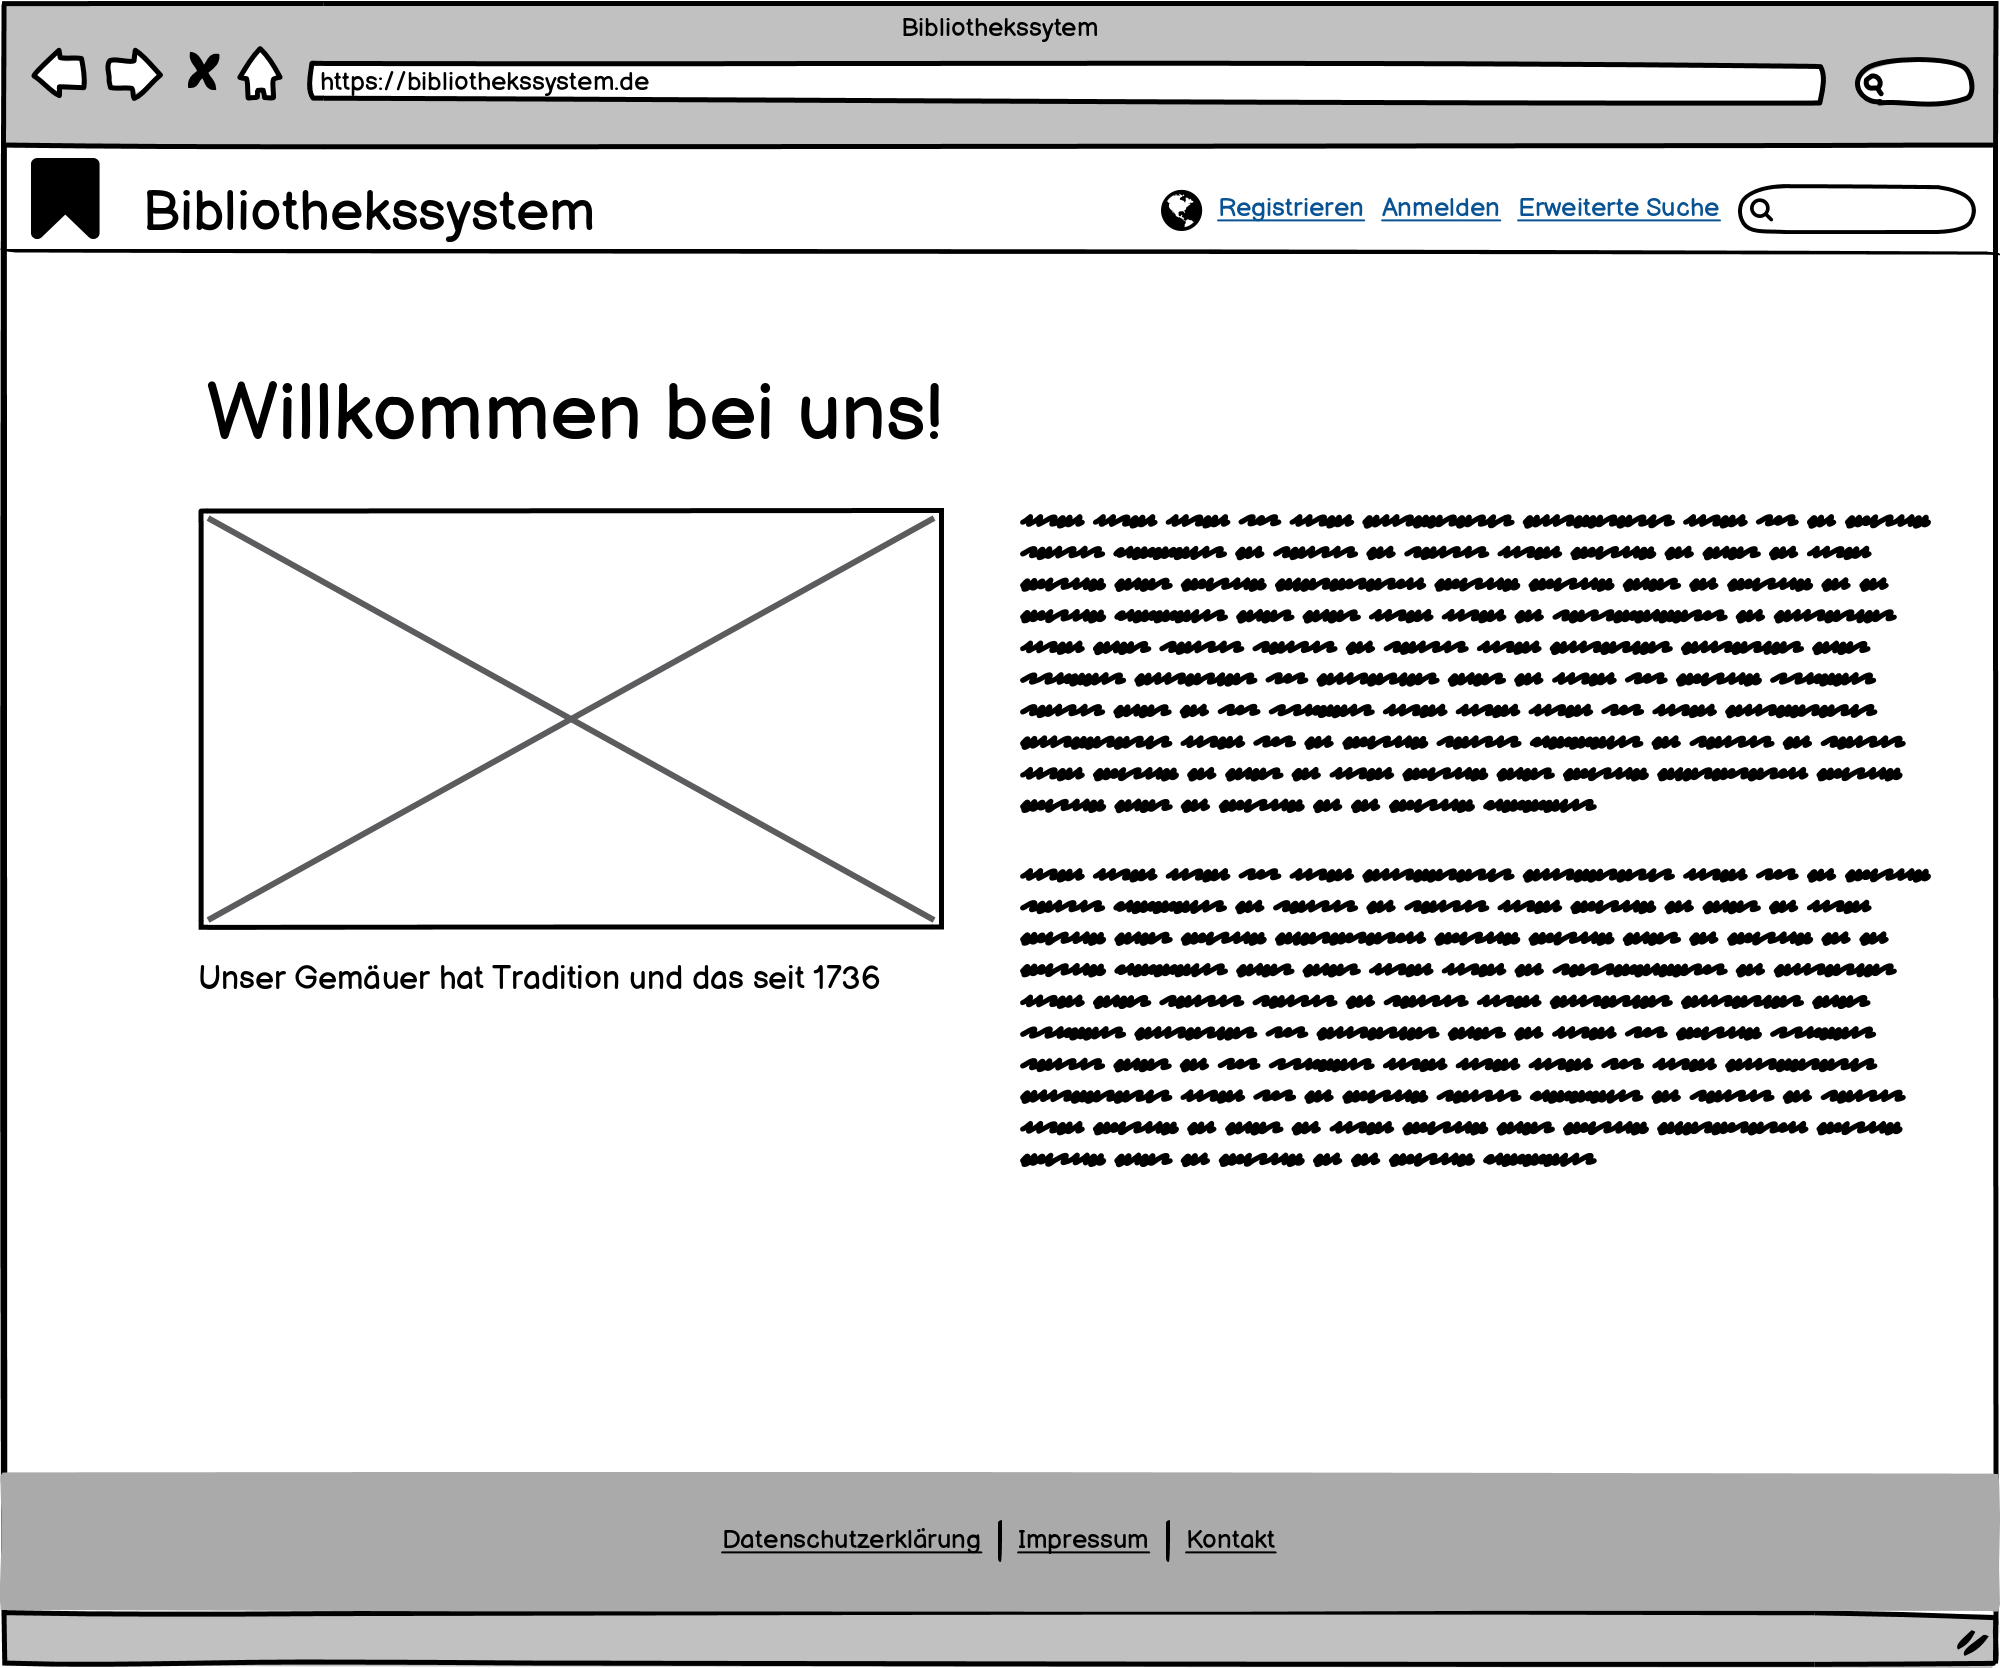
\includegraphics[width = 40em]{Startseite}
    \caption{Skizzierung der Startseite}
    \label{startseite}
\end{figure}

\begin{figure}[h]
    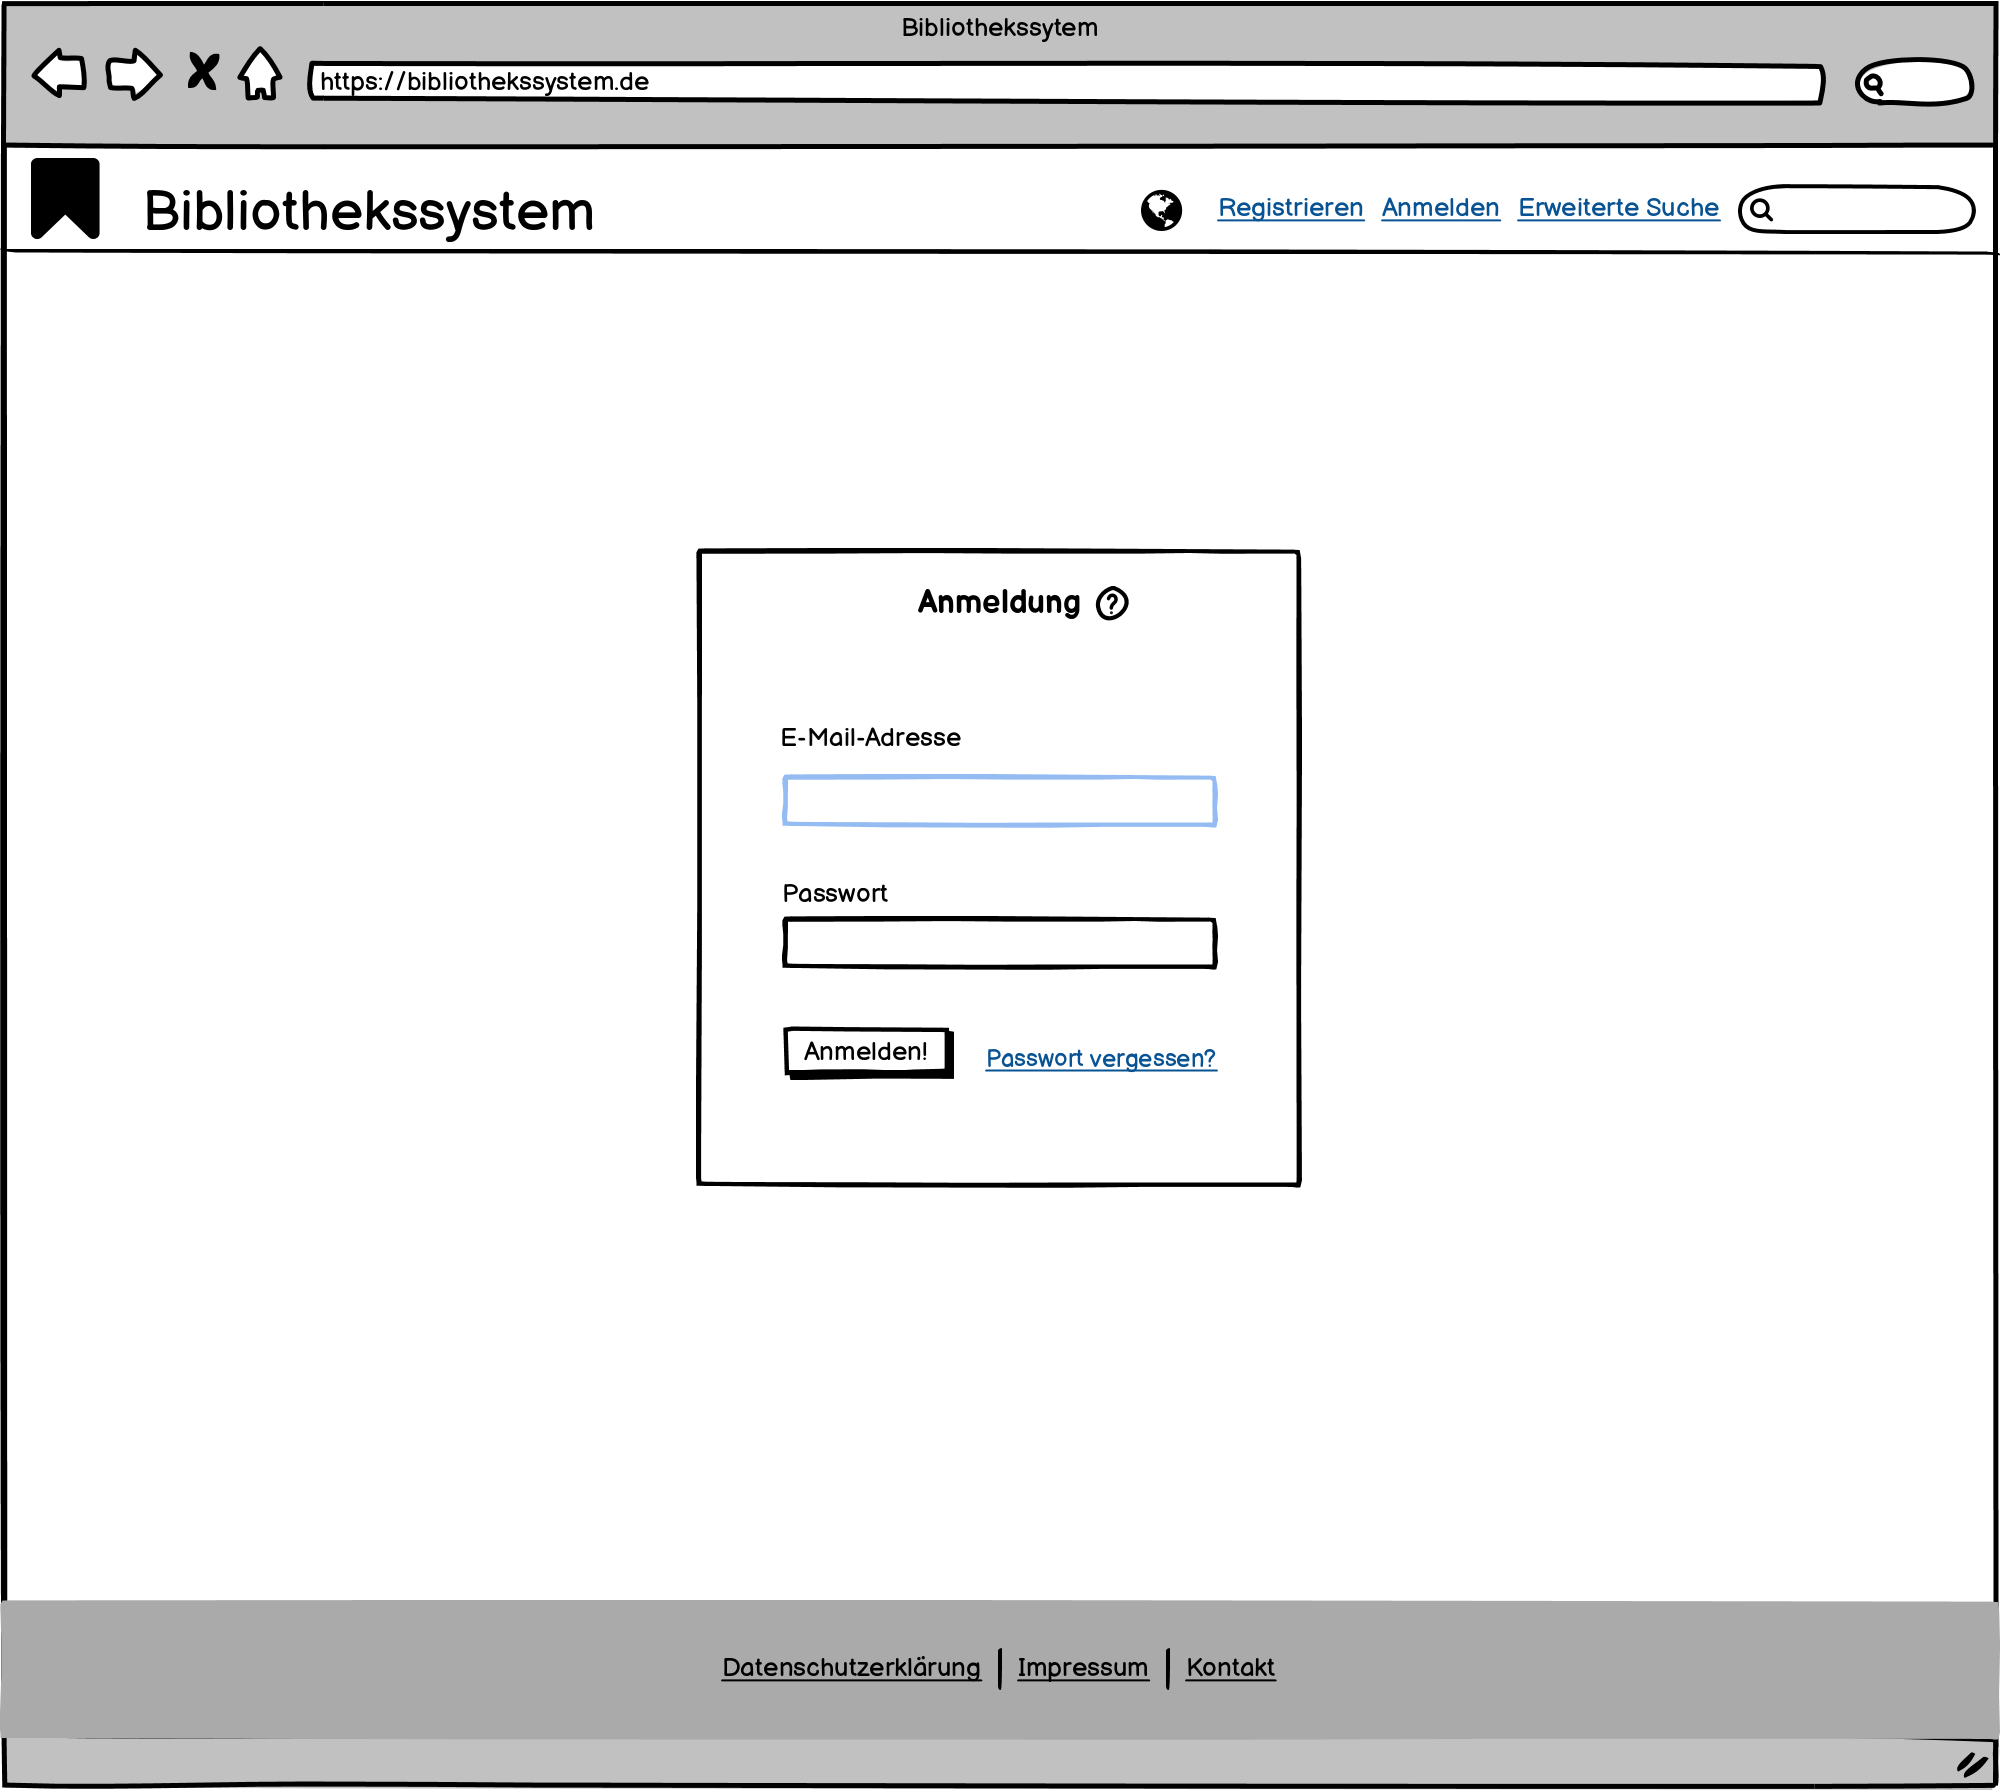
\includegraphics[width = 40em]{Anmeldemaske}
    \caption{Skizzierung der Anmeldemaske}
    \label{anmeldemaske}
\end{figure}

\begin{figure}[h]
    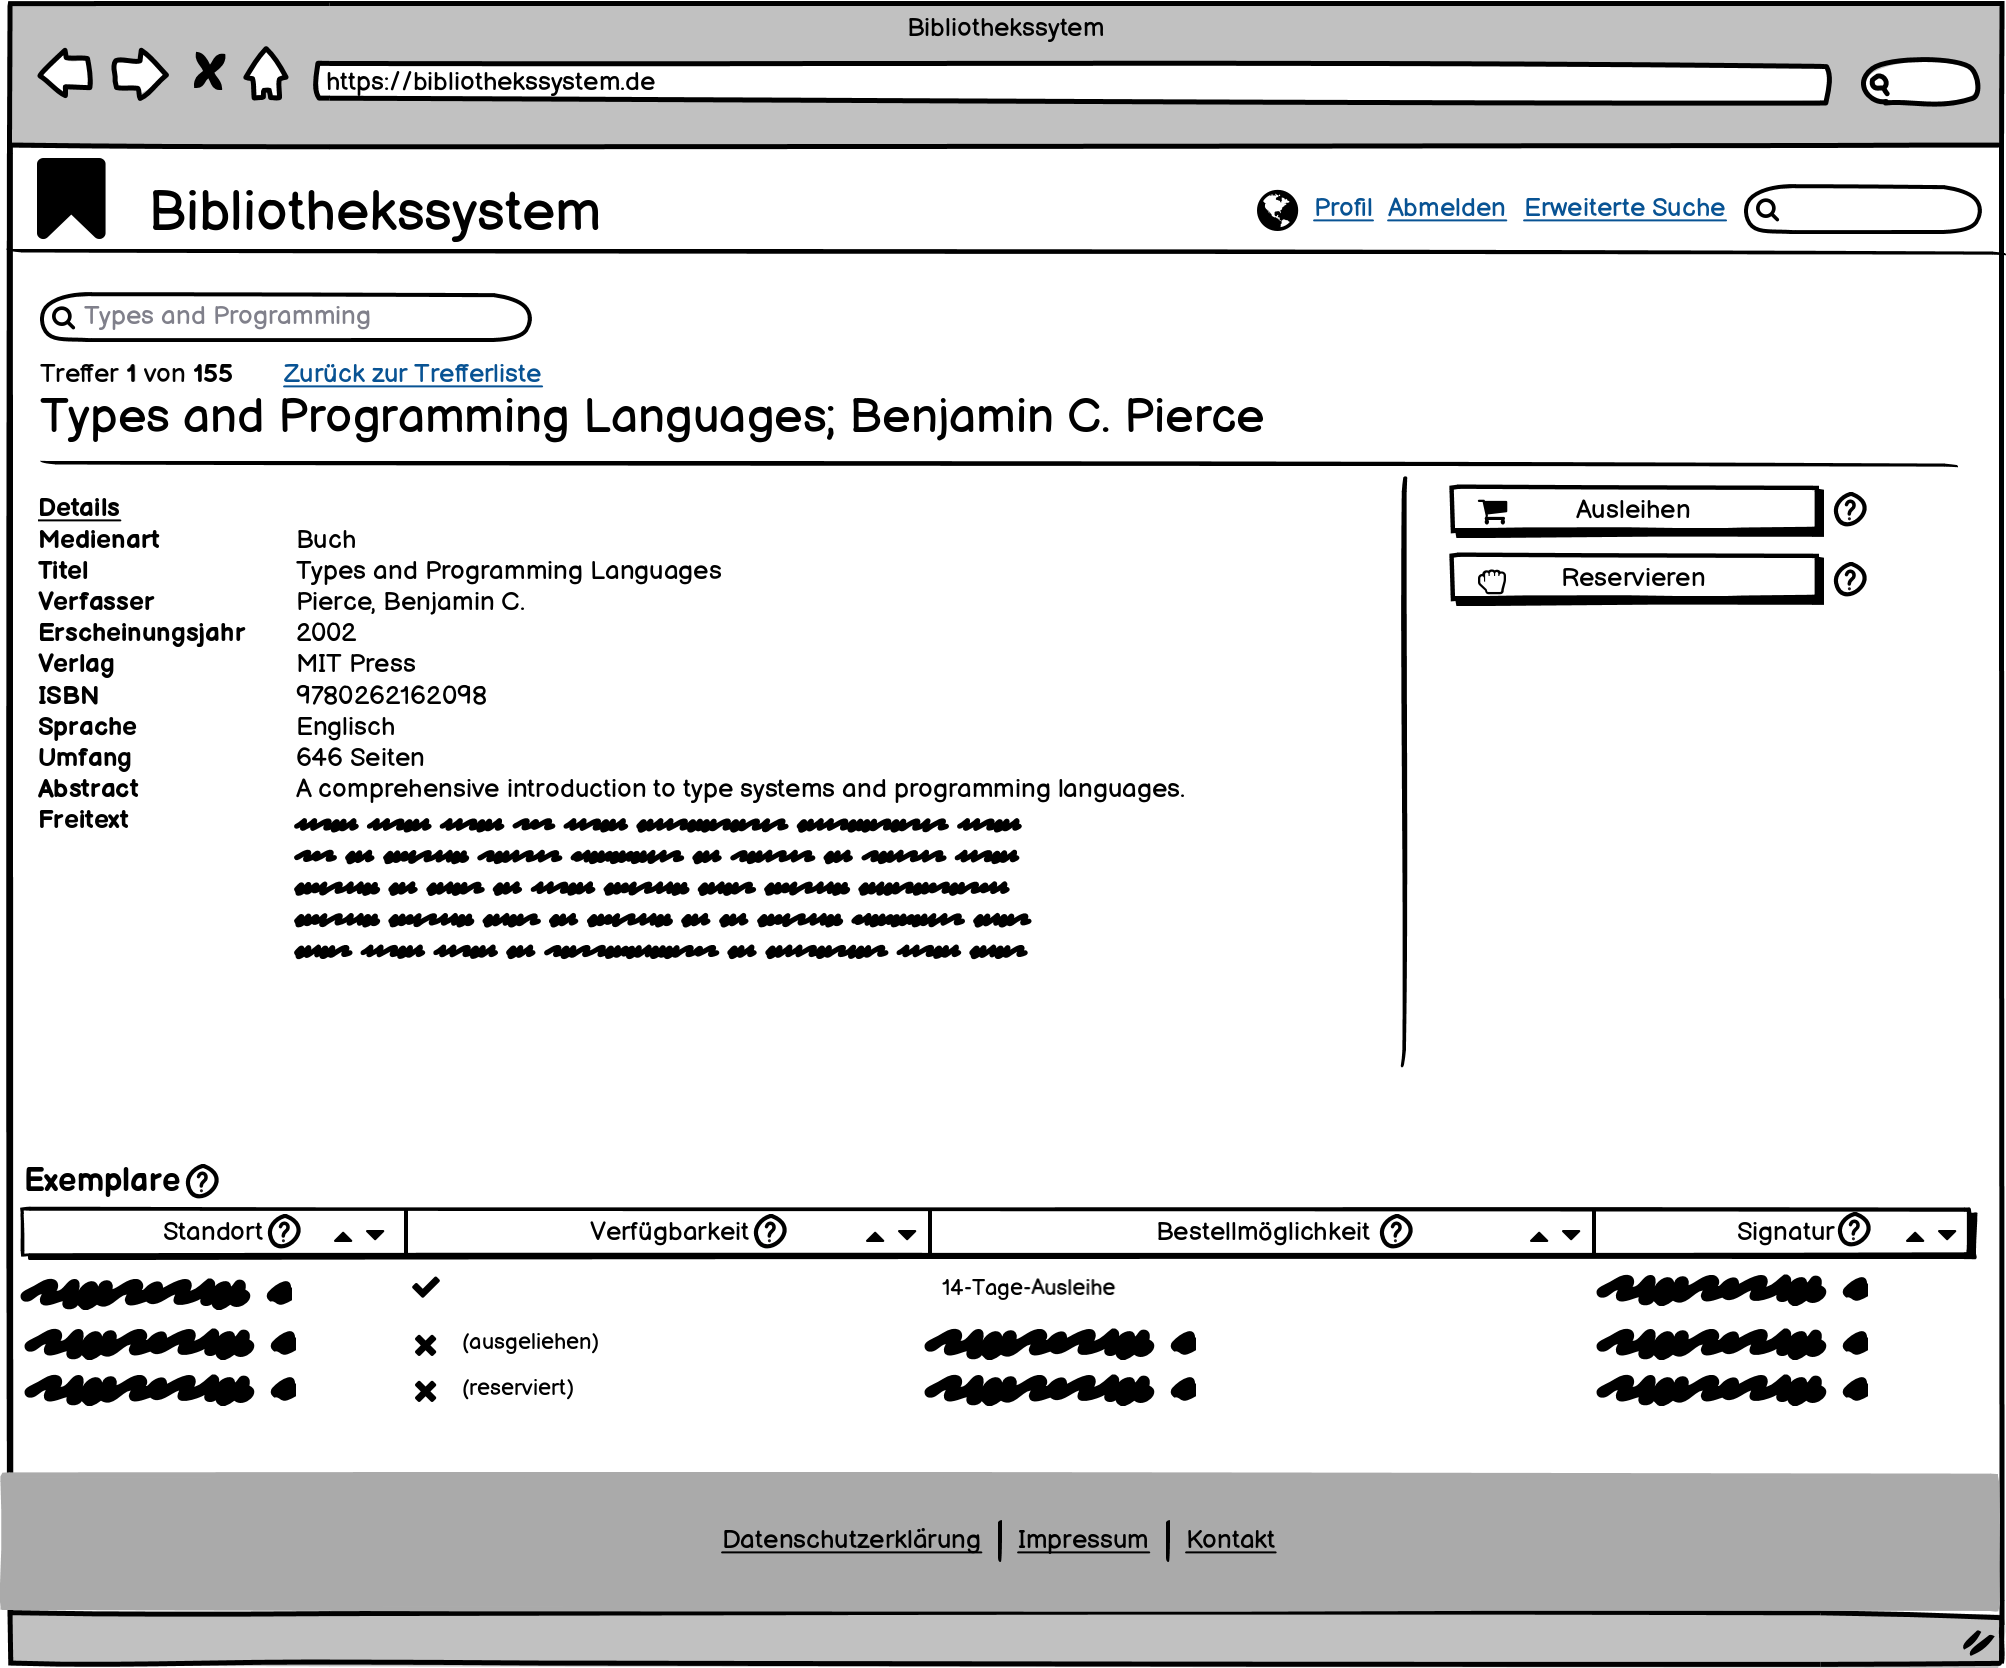
\includegraphics[width = 40em]{Mediumsseite}
    \caption{Skizzierung der Mediumsseite aus Sicht eines nicht privilegierten Nutzers}
    \label{mediumsseite_angemeldet}
\end{figure}

\begin{figure}[h]
    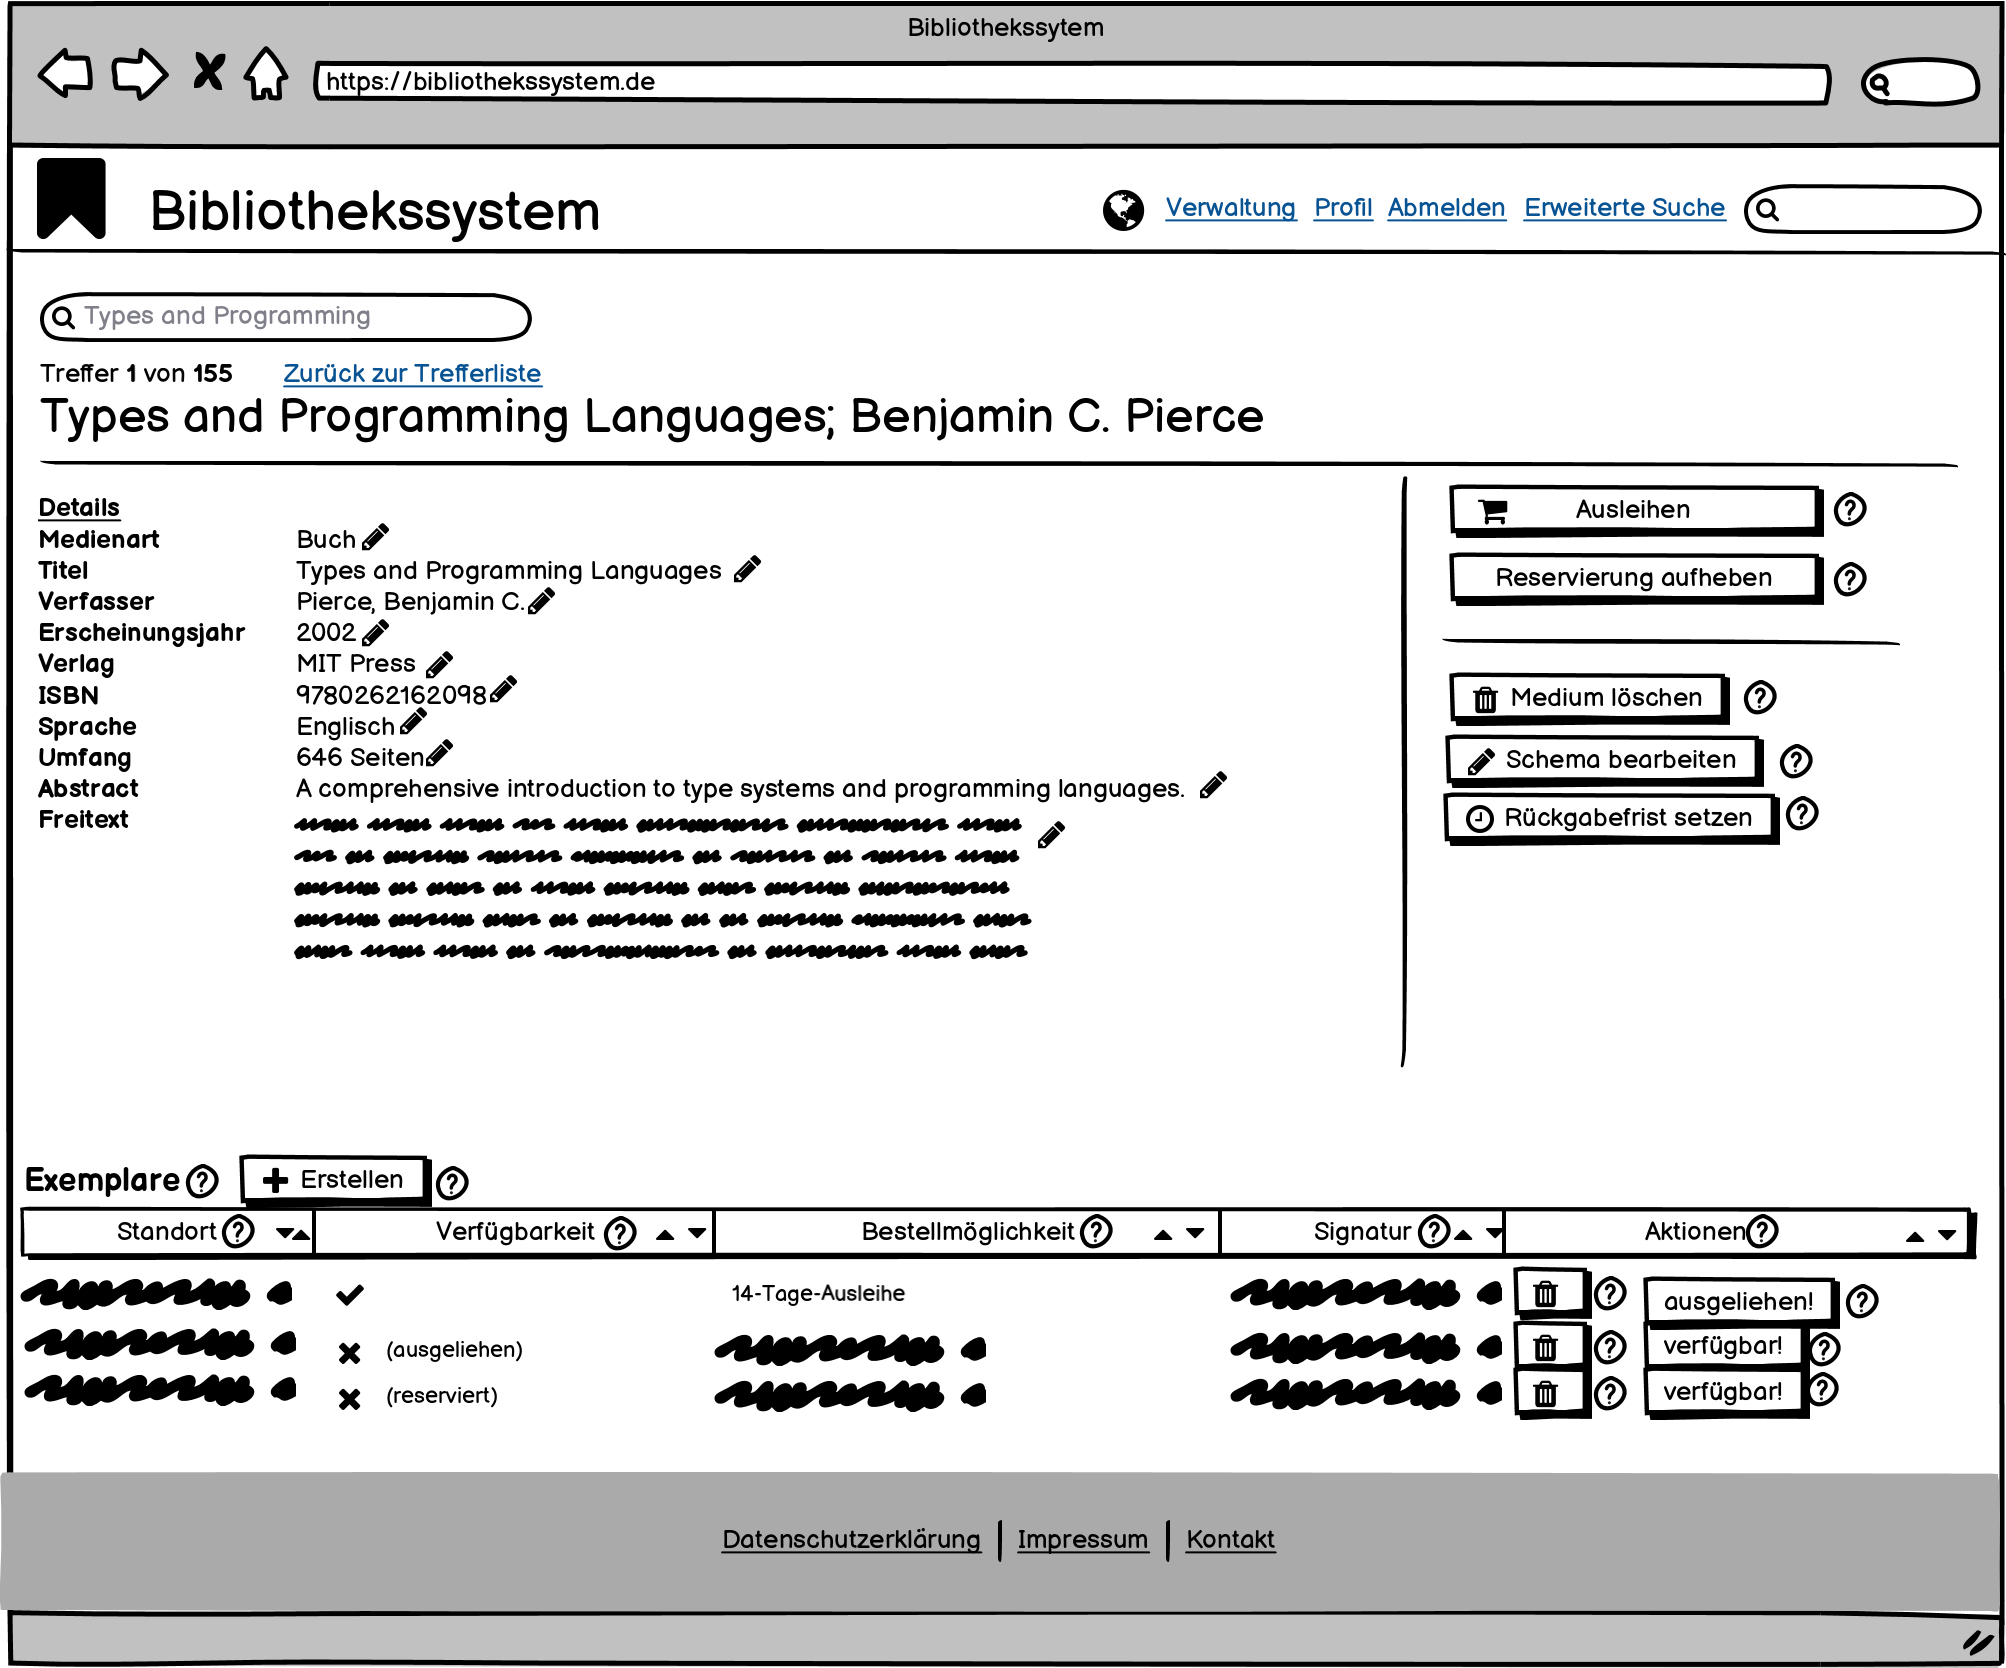
\includegraphics[width = 40em]{Mediumsseite_Admin}
    \caption{Skizzierung der Mediumsseite aus Sicht eines Administrators}
    \label{mediumsseite_admin}
\end{figure}

\newpage
\newgeometry{left=0.1cm,right=0.1cm,top=0.1cm,bottom=0.1cm}

\begin{figure}[h]
    \centering
    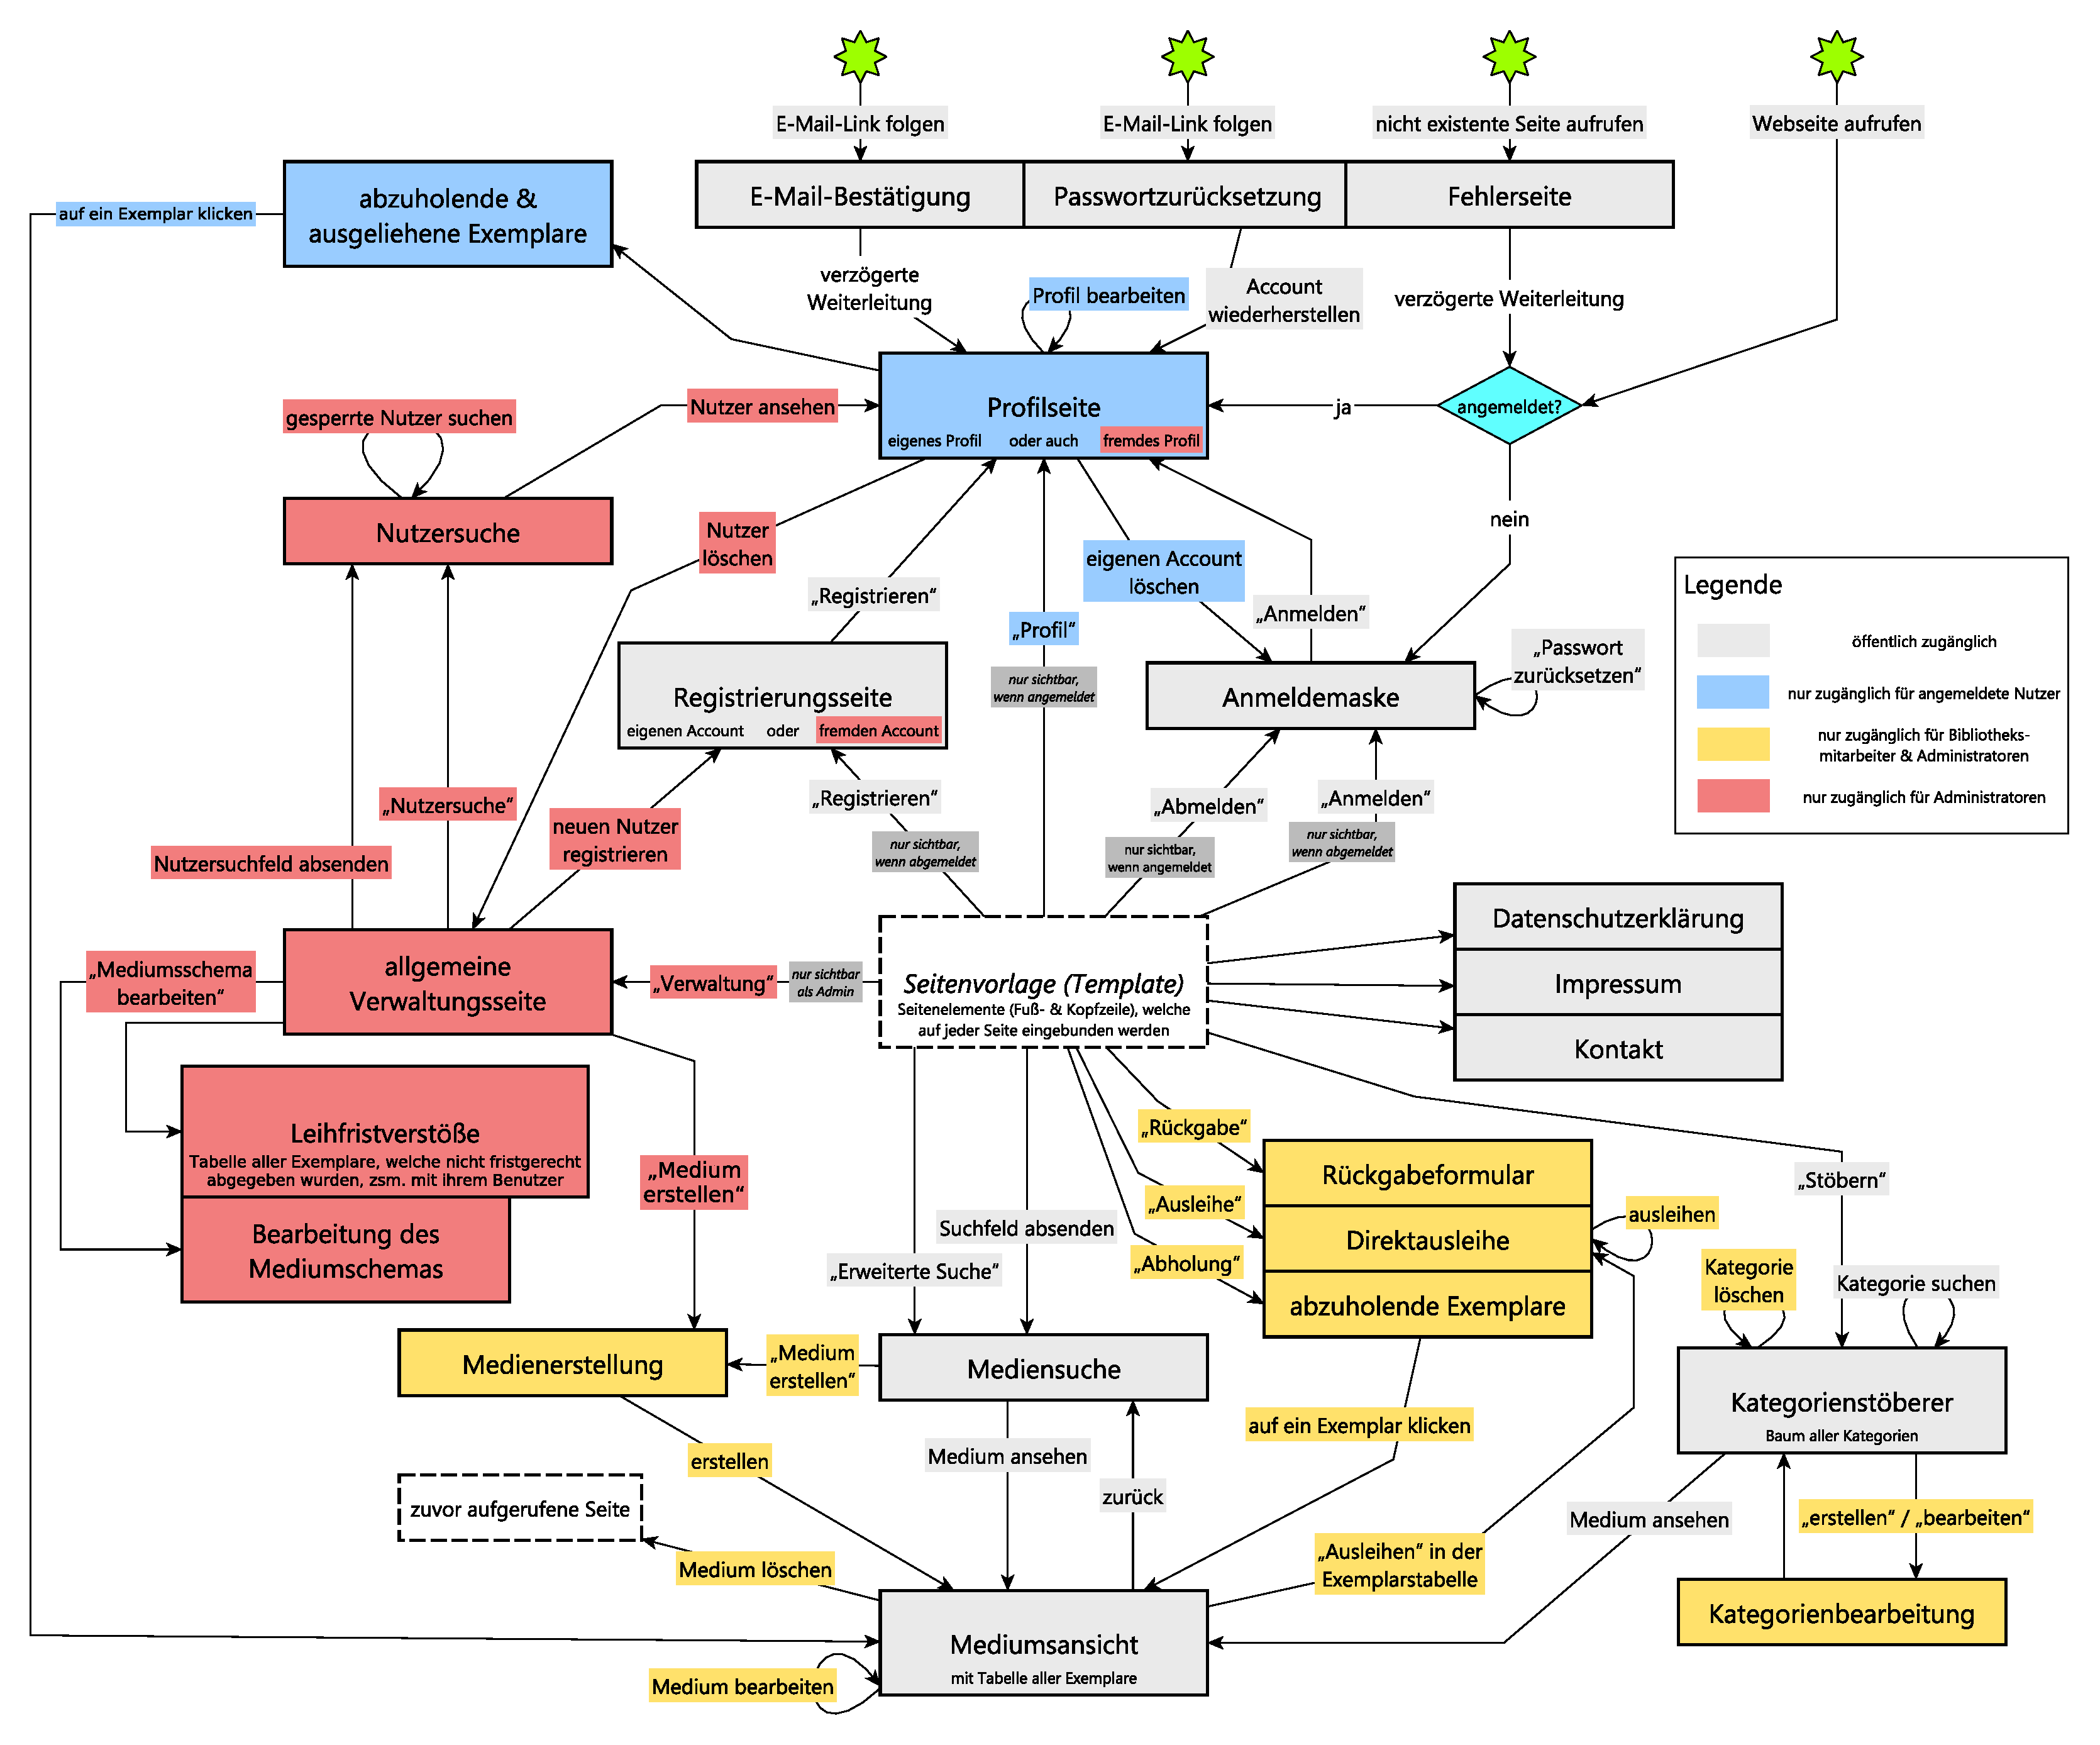
\includegraphics[angle = 270, width = 40em]{site_map}
    \caption{Die Inhaltsübersicht der Webseite (engl. \textit{site map})}
    \label{site_map}
\end{figure}

\restoregeometry
\newpage

\section{Qualitätsanforderungen} %-------------------------------------------------------------------------------------------------
\sectionauthor{Mohamad Najjar}

Die folgende Tabelle zeigt die Priorität, die jeder Qualitätsanforderung zugewiesen wird.
	
\begin{center}
\begin{tabular}{ |l||c|c|c|c| } 
 \hline
  & sehr wichtig & wichtig & weniger wichtig & unwichtig \\
 \hline\hline
 Benutzerfreundlichkeit & X & & & \\
 \hline
 Funktionalität & X & & & \\ 
 \hline
 Korrektheit & X & & & \\
 \hline
 Robustheit & & X & & \\
 \hline
 Vertrauenswürdigkeit & & X & & \\
 \hline
 Effizienz & & X & & \\
 \hline
 Änderbarkeit & & X & & \\
 \hline
 Portierbarkeit & & &  & X \\

 \hline
\end{tabular}
\end{center}
\begin{itemize}
\item Da  unser System einfach und intuitiv zu bedienen sein soll und die häufigsten Funktionen sollten
 zugänglich sein, wird sehr wichtig  auf die Benutzerfreundlichkeit und Funktionalität gesetzt.
\item Aus dem Grund, dass sensible Daten zu jedem Zeitpunkt nur für Berechtigte zugänglich sind, wird auf  wichtig gesetzt.
\item Um nachträgliche Änderungen und Erweiterungen einfach vornehmen zu können, 
sollte das System in gewissen Grenzen flexibel genug sein.
\item Um Manipulationen mit bekannten Angriffsmethoden zu verhindern, werden bestimmte Maßnahmen getroffen.
\end{itemize}

\newpage

\section{Testing} %-------------------------------------------------------------------------------------------------
\sectionauthor{Sergei Pravdin}
Das Bibliothekssystem ist erfolgreich installiert, somit sind ein Administrator, ein registrierten Benutzer und ein Medium eingesetzt. Das System befindet sich im offenen Modus, deshalb ist die Registrierung für die allen E-Mail-Domänen möglich.
\subsection{Nutzerverwaltung}
		\subsubsection{Administrator}
			\specification{T}{010}{Das System wurde vom Administrator ins geschlossene Modus umgeschaltet. Ein anonymer Benutzer ruft die Katalog-Seite auf, aber eine Anmeldungsseite wird geladen.­­­­­ (\hyperlink{spec:F:10}{/F10/}) }
			\specification{T}{020}{Der Administrator erlaubte die Registrierung nur für die Domäne "@fim.uni-passau.de". 
				Ein anonymer Benutzer befindet sich auf der Seite Registrierung und gibt Angaben, inkl. eine E-Mail mit der Domäne "@gmail.com", in den Formular an und klickt ein Button "Registrieren". 
				Eine entsprechende Fehlermeldung wird angezeigt. (\hyperlink{spec:F:20}{/F20/}) }
			\specification{T}{030}{Ein anonymer Benutzer befindet sich auf der Seite Registrierung und gibt valide Angaben in den Formular an und klickt aufs Button "Registrieren". 
				Eine entsprechende Meldung wird gezeigt, dass der Benutzer seine E-Mail-Adresse bestätigen muss. Die Registrierung wird abgeschlossen, falls die E-Mail-Adresse verifiziert wird. (\hyperlink{spec:F:90}{/F90/}) }
			\specification{T}{40}{Der Administrator befindet sich auf einer Konto-Seite eines Benutzers und ändert ein Vorname des Benutzers. Somit wird ein neuer Vorname des Benutzers auf seiner Konto-Seite sichtbar. (\hyperlink{spec:F:40}{/F40/}) }
			\specification{T}{50}{Der Administrator löscht einen Benutzer. Der Benutzer befindet sich auf der Anmeldungsseite und versucht sich mit seinem Login und seinem Kennwort anzumelden. Eine entsprechende Fehlermeldung wird gezeigt.
				(\hyperlink{spec:F:50}{/F50/}) } 
			\specification{T}{60}{Der Administrator gibt einen Name eines existierenden Benutzers ins Suchfeld an. Der entsprechende Benutzer wird gezeigt. (\hyperlink{spec:F:60}{/F60/}) }
			\specification{TW}{70}{Der Administrator verbietet die Ausleihe-Funktion eines Benutzers. Der Benutzer befindet sich auf einer Seite eines Mediums und klickt aufs Button "Buchen". Eine entsprechende Fehlermeldung wird gezeigt. 
				(\hyperlink{spec:W:70}{/W70/}, \hyperlink{spec:W:100}{/W100/}) }
			\specification{TW}{80}{Ein Benutzer wurde von einem Administrator gesperrt, somit darf er keine Medien ausleihen. Der Administrator ruft eine Seite von gesperrten Konten auf. Der gesperrte Benutzer ist in der gezeigten Liste sichtbar. 
				(\hyperlink{spec:W:80}{/W80/}) }
			\subsubsection{Anonyme Nutzer}
			\specification{T}{90}{Ein anonymer Benutzer befindet sich auf der Seite Registrierung und gibt valide Angaben in den Formular an und klickt aufs Button "Registrieren".
				Eine entsprechende Meldung wird gezeigt, dass der Benutzer seine E-Mail-Adresse bestätigen muss. Die Registrierung wird abgeschlossen, falls die E-Mail-Adresse verifiziert wird. (\hyperlink{spec:F:90}{/F90/}) }
		\subsubsection{Registrierte Nutzer}
			\specification{T}{100}{Ein Benutzer befindet sich auf der Anmeldungsseite und gibt sein Login und sein Kennwort ins Formular an. Eine Seite mit de angemeldeten Benutzer wird geladen. (\hyperlink{spec:F:100}{/F100/}) }
			\specification{T}{110}{Ein angemeldeter Benutzer befindet sich auf einer irgendwelchen Seite des Systems und klickt auf den Button "Abmelden".
				Die Seite wird wiedergeladen und der Benutzer ist nicht mehr angemeldet, somit ist der Button "Anmelden" sichtbar. (\hyperlink{spec:F:110}{/F110/}) }
		\subsubsection{Angemeldete Nutzer}
			\specification{T}{120}{Ein Benutzer befindet sich auf seiner Konto-Seite. Er klickt auf den Button "Editieren" und verändert sein Geburtsdatum, dann klickt er auf den Button "Speichern". 
				Somit ist sein neues Geburtsdatum auf der Konto-Seite sichtbar. (\hyperlink{spec:F:120}{/F120/}) }
			\specification{T}{130}{Ein Benutzer befindet sich auf seiner Konto-Seite. Er klickt auf den Button "Konto löschen". Eine Meldung wird gezeigt und der Benutzer bestätigt das Löschen.
				Das Konto wird gelöscht und die Startseite des Systems wird geladen. (\hyperlink{spec:F:130}{/F130/}) }
			\specification{TW}{140}{Ein Benutzer befindet sich auf seiner Konto-Seite. Er klickt auf den Button "Bild hochladen" und wählt aus seinem Rechner ein Bild aus. 
				Er klickt den Button "einsetzen" und ein Bild wird eingesetzt und ist auf der Konto-Seite sichtbar. (\hyperlink{spec:W:140}{/W140/}) }
		\subsubsection{Alle Nutzer}
			\specification{T}{150}{Ein Benutzer befindet sich auf der Registrierung-Seite und gibt einen invaliden Name und eine invalide E-Mail-Adresse.
				Eine entsprechende Fehlermeldung über die beiden Fehler wird gezeigt. (\hyperlink{spec:W:150}{/W150/}) }
\subsection{Navigation \& Suche}
		\subsubsection{Alle Nutzer}
			\specification{T}{160}{Der Benutzer gibt eine Texteingabe ins Suchfeld und sucht Medien nach einer Kategorie. Entsprechende der gewünschten Kategorie Medien werden gezeigt. (\hyperlink{spec:F:160}{/F160/}, \hyperlink{spec:F:180}{/F180/}) }
			\specification{T}{170}{Der Benutzer befindet sich auf der Baum-Darstellung-Seite von allen Kategorien und klickt auf eine Kategorie. Entsprechende der gewünschten Kategorie Medien werden gezeigt. (\hyperlink{spec:F:170}{/F170/}) }
			\specification{T}{180}{Der Benutzer befindet sich auf der Katalog-Seite und klickt auf ein Medium. Eine Seite des Mediums mit einer Liste von allen Exemplaren wird geladen. (\hyperlink{spec:F:190}{/F190/}) }
			\specification{T}{190}{Der Benutzer befindet sich auf der Katalog-Seite und klickt auf eine Spalte. Medien werden nach dieser Spalte sortiert. (\hyperlink{spec:F:200}{/F200/}) }
			\specification{T}{200}{Der Benutzer befindet sich auf irgendwelcher Seite des Systems. Er klickt auf den Button "Impressum" und eine Impressum-Seite wird geladen. Die Kontaktdaten sind sichtbar. (\hyperlink{spec:F:210}{/F210/}) }
			\specification{TW}{210}{Der Benutzer befindet sich auf der Katalog-Seite und setzt ein, dass max. 10 Medien auf einer Seite sichtbar sein dürfen. 
				Die Katalog-Seite wird wieder geladen und max. 10 Medien sind sichtbar. (\hyperlink{spec:W:230}{/W230/})}
			\subsection{Ausleihe \& Rückgabe}
		\subsubsection{Administrator}
			\specification{T}{220}{Der Administrator setzt den Zeitabstand als 2 Minute zwischen dem automatischen Versenden einer E-Mail-Mahnung und der Rückgabefrist für ein Medium an. 
				Außerdem setzt er einen Rückgabefrist des Mediums als 1 Minute. Der Personalarbeiter bucht für einen Benutzer das Medium im System, gibt es ab und in 2 Minuten bekommt der Benutzer eine E-Mail-Mahnung. 
				In seinem Konto ist eine Meldung über eine Mahnung bei diesem Medium sichtbar. (/F230/, /F250/, /F260/)}
			\specification{T}{230}{Der Administrator setzt den Zeitabstand zwischen der Initiierung eines Ausleihvorgangs durch einen Nutzer und dem Abschluss dieser Initiierung durch einen Personalarbeiter oder Administrator 
				und die maximale Reservierungsdauer an. Ein Benutzer bucht ein Medium im System. Ein Button "Buchen" ist nicht mehr für andere Benutzer sichtbar. 
				Ein Button "Reservieren" ist für andere Benutzer sichtbar. (/F240/, /W280/, /F300/)}
			\specification{T}{240}{Der Administrator ruft eine Liste von Benutzern, die einen Rückgabefrist überschritten haben, an. Entsprechende Liste von Benutzern ist sichtbar. (/F270/)}
		\subsubsection{Personalarbeiter}
			\specification{T}{250}{Der Personalarbeiter ruft eine Liste von zur Abholung markierten Exemplaren an. Entsprechende Exemplaren sind sichtbar. (/F290/)}
			\specification{T}{260}{Der Personalarbeiter befindet sich auf einer Medium-Seite und klickt auf den Button "Freigeben" bei einem Exemplar. 
				Ein angemeldeter Benutzer befindet sich auf der Seite dieselben Medium und der Button "Buchen" ist für ihn sichtbar. (/F310/)}
		\subsubsection{Registrierte Nutzer}
			\specification{T}{270}{Ein angemeldeter Benutzer befindet sich auf einer Medium-Seite und klickt auf den Button "Buchen". Eine entsprechende Meldung über eine erfolgreiche Buchung wird gezeigt. (/F320/) }
			\specification{TW}{280}{Ein angemeldeter Benutzer befindet sich auf einer Seite eines Mediums, das ausgeliehen ist, und klickt auf den Button "Reservieren". 
				Eine entsprechende Meldung über eine erfolgreiche Reservierung wird gezeigt. (/W330/) }
			\specification{TW}{290}{Ein angemeldeter Benutzer befindet sich auf einer Seite eines Mediums, das von ihm reserviert wurde, und klickt auf den Button "Reservierung widerrufen". 
				Eine entsprechende Meldung über eine erfolgreiche Widerrufung der Reservierung wird gezeigt. (/W340/) }
\subsection{Katalogführung}
		\subsubsection{Administrator}
			\specification{T}{300}{Der Administrator befindet sich auf der Seite aller Kategorien. Er klickt auf den Button "Erstellen" und gibt einen Name einer neuen Kategorie an und speichert. 
				Die Seite wird wiedergeladen und die neue Kategorie sichtbar. (/F350/) }
			\specification{T}{310}{Der Administrator befindet sich auf der Seite aller Kategorien. Er klickt auf den Button "Löschen" bei einer Oberkategorie. Eine entsprechende Meldung wird gezeigt und das Löschen vom Administrator bestätigt. 
				Die Seite wird wiedergeladen und die gelöschte Kategorie ist nicht mehr auf der Seite sichtbar. (/F360/) }
			\specification{T}{320}{Der Administrator befindet sich auf der Katalog-Seite und klickt auf den Button "Medium erstellen". Ein entsprechendes Formular wird gezeigt, der Administrator gibt die Angaben eines Mediums an und speichert. 
				Die Seite wird wiedergeladen und ein erstelltes Medium ist sichtbar. (/F370/)}
			\specification{T}{330}{Der Administrator befindet sich auf der Katalog-Seite und klickt auf den Button "Löschen" bei einem Medium. Eine entsprechende Meldung wird gezeigt und das Löschen vom Administrator bestätigt. 
				Die Seite wird wiedergeladen und das gelöschte Medium ist nicht mehr auf der Seite sichtbar. (/F380/) }
			\specification{T}{340}{Der Administrator befindet sich auf der Medium-Seite und klickt auf den Button "Exemplar erstellen". Ein entsprechendes Formular wird gezeigt, der Administrator gibt die Angaben eines Exemplars an und speichert. 
				Die Seite wird wiedergeladen und ein erstelltes Exemplar ist sichtbar. (/F390/)}
			\specification{T}{350}{Der Administrator befindet sich auf der Medium-Seite und klickt auf den Button "Exemplar löschen". 
				Das Exemplar ist nicht ausgeliehen, deshalb wird die Seite ohne Meldung wiedergeladen und ein erstelltes Exemplar ist nicht mehr sichtbar. (/F400/)}
	\subsection{Weitere Personalisierungen}
		\subsubsection{Administrator}
			\specification{T}{360}{Der Administrator befindet sich auf der Einstellungen-Seite und klickt auf den Button "Name der Organisation ändern". Dann gibt er einen neuen Name an und speichert. 
				Die Seite wird wiedergeladen und der neue Name ist auf der Seite sichtbar. (/F410/) }
			\specification{T}{370}{Der Administrator befindet sich auf der Einstellungen-Seite und klickt auf den Button "Logo hochladen". Dann wählt er ein Bild aus seinem Rechner aus und speichert. 
				Die Seite wird wiedergeladen und das Logo ist auf der Seite sichtbar. (/F420/)}
			\specification{T}{380}{Der Administrator befindet sich auf der Einstellungen-Seite und klickt auf den Button "Farbe ansetzen". Dann wird eine Liste der Farben gezeigt und der Administrator wählt eine Farbe aus. 
				Die Seite wird wiedergeladen und die ausgewählte Farbe ist auf der Seite sichtbar. (/F430/)}
			\specification{T}{390}{Der Administrator befindet sich auf der Impressum-Seite und klickt auf den Button "Ändern". Dann gibt er eine neue Kontaktnummer an und speichert. 
				Die Impressum-Seite wird wiedergeladen und die neue Kontaktnummer ist auf der Seite sichtbar. (/F440/)}
		\subsubsection{Alle Nutzer}
			\specification{TW}{400}{Der Benutzer befindet sich auf irgendwelcher Seite des Systems und klickt auf Button "Sprache wechseln". 
				Dann wird er eine englische Sprache ausgewählt und die Seite wird auf der englischen Sprache wiedergeladen. (/W450/) }

\newpage

\section{Entwicklungsumgebung} %-------------------------------------------------------------------------------------------------
\sectionauthor{Jonas Picker}

Die Entwicklung finden auf verschiedenen Privatrechnern der Teammitglieder statt, deren Bauteile und Betriebssysteme in den folgenden Listen kurz umrissen werden, keiner der Rechner weißt sonstige Besonderheiten auf. 

\subsection{Software}

\begin{itemize}
\item \underline{\textbf{Dokumentenbearbeitung}}: 
\begin{flushleft}
LaTeX Distribution MiKTeX, Version: 21.2 \linebreak
Overleaf Online Latex Editor \linebreak
LaTeX Distribution MacTeX-2021 \linebreak
\end{flushleft}
\item \underline{\textbf{Webbrowser}}:
\begin{flushleft}
Google Chrome, Version: 88.0 \linebreak
Mozilla Firefox, Version: 85.0 \linebreak
Apple Safari, Version: 14.0.3 \linebreak
\end{flushleft}
\item \underline{\textbf{Integrierte Entwicklungsumgebungen}}: 
\begin{flushleft}
Eclipse IDE for Enterprise Java Developers, Version: 2020-12 (4.18.0) \linebreak
IntelliJ IDEA 2021.1 Ultimate Edition \linebreak
\end{flushleft}
\item \underline{\textbf{Objektorientierte Modellierung}}: 
\begin{flushleft}
IBM Rational Software Architect Designer 9.7 \linebreak
\end{flushleft}
\item \underline{\textbf{Programmiersprachen, Entwicklungs- \& Testframeworks}}: 
\begin{flushleft}
Java OpenJDK JDK 16 GA-Release\linebreak
Jakarta EE 9 \linebreak
Jakarta Server Faces 3.0 Mojarra Implementation \linebreak
CDI 3.0 with Red Hat Weld, Version: 4.0.1.Final \linebreak
Cascading Style Sheets Level 3 \linebreak
JUnit Platform, Version: 1.7.1 \linebreak
Selenium Server (Grid), Version: 3.141.59 \linebreak
\end{flushleft}
\item \underline{\textbf{Versionsmanagement}}:
\begin{flushleft}
git, Version 2.31.1 \linebreak
\end{flushleft}
\item \underline{\textbf{Betriebssysteme der Entwicklungsrechner}}:
\begin{flushleft}
MacOS Big Sur, Versionen: 11.2.3 und 11.2.1 \linebreak
Windows 10 Home 20H2 \linebreak
GNU/Linux Arch, Version: 5.11.11 \linebreak
GNU/Linux Debian, Version: 4.19.132-1 \linebreak
\end{flushleft}
\item \underline{\textbf{Graphische Prototypenbearbeitung}}:
\begin{flushleft}
Balsamiq Wireframes, Version: 4.2.4 \linebreak 
yEd Graph Editor, Version: 3.21.1 \linebreak 
\end{flushleft}
\item \underline{\textbf{Applikationsserver}}: 
\begin{flushleft}
Apache Tomcat, Version: 10.0.2 \linebreak
\end{flushleft}
\item \underline{\textbf{Datenbanktreiber und Visualisierung}}: 
\begin{flushleft}
PostgreSQL JDBC 4.2 Driver, Version: 42.2.19 \linebreak
DBeaver, Version: 21.0.2
\end{flushleft}
\item \underline{\textbf{Teamkommunikation}}: 
\begin{flushleft}
Slack \linebreak
Discord \linebreak
Skype \linebreak
Stud.IP \linebreak
\end{flushleft}
\end{itemize}

\subsection{Hardware}

\begin{itemize}
\item \underline{\textbf{Entwicklungsrechner}}: 
\begin{flushleft}
MacBook Pro, 8GB RAM, Intel Core i5 2GHz  \linebreak
HP Laptop 15-db1xxx, 16GB RAM, AMD Ryzen 5 3500U 2.1GHz \linebreak
2x MacBook Pro, 8GB RAM, Intel Core i5 2.3GHz \linebreak
Tower-PC, 16GB RAM, AMD Ryzen 5 3600XT 3.8GHz \linebreak
\end{flushleft}
\item \underline{\textbf{Referenzrechner}}:
\begin{flushleft}
CIP-Pool Computer 'schratz', Uni Passau, 15.6GB RAM, Intel Core i7-4790 3.60GHz CPU, Intel I217-LM Ethernet Controller \linebreak
Spezifikation der virtualisierten Datenbank (siehe Entwicklungsschnittstellen) bezieht sich auf die Referenzhardware von 'schratz' und besitzt eine geschätze Übertragungsrate von ca. 1GB/s ins Internet. Die Datenbank unterstützt das Verschlüsselungsprotokoll TLS mit einem Zertifikat. \linebreak
\end{flushleft}
\end{itemize}

\subsection{Entwicklungsschnittstellen}

\begin{itemize}
\item \begin{flushleft} Netzwerk- und Internetverbindung \end{flushleft} 
\item \begin{flushleft} Virtuelle private Netwerkanbindung mit OpenVPN, Version 2.5.1 \end{flushleft} 
\item \begin{flushleft} Git-verwaltetes Repository der Uni Passau, Website: https://git.fim.uni-passau.de/ \end{flushleft} 
\item \begin{flushleft} Virtualisierte Datenbank der Uni Passau, Hostname: bueno.fim.uni-passau.de \end{flushleft}
\end{itemize}

\newpage

\section{Glossar} %-------------------------------------------------------------------------------------------------
\sectionauthor{Jonas Picker}
	\begin{itemize}
		\item OPAC - Online public access catalog
	\end{itemize}

\end{document}
